\documentclass{beamer}
\usetheme{Madrid}
\usecolortheme{default}
\usepackage[T1]{fontenc}
\usepackage[french]{babel}
\usepackage{graphicx}
\usepackage{amsmath}
\usepackage{amssymb}
\usepackage{mathrsfs}
\usepackage{subfigure}
\usepackage{empheq}

% Ajouter le plan en haut
\useoutertheme{infolines}
\setbeamertemplate{headline}{
	\begin{beamercolorbox}[ht=2.25ex,dp=3.75ex]{section in head/foot}
		\insertnavigation{\paperwidth}
\end{beamercolorbox}}

\title[]
{Sécurisation de batiment par amortisseur harmonique}

\subtitle{}

\author{FRAMBOURT Mateïs} % (optional, for multiple authors)




\date[N°42185] % (optional)
{Numéro de candidat:\\ 42185}

%\logo{\includegraphics[height=0.8cm]{logo_uoft}}

\definecolor{uoftblue}{RGB}{6,41,88}
\setbeamercolor{titlelike}{bg=uoftblue}
\setbeamerfont{title}{series=\bfseries}
\setbeamertemplate{caption}[numbered]
\begin{document}
	
	\frame{\titlepage}
	%En Binôme avec BOCQUILLON Noé
	\section{Préambule}
	\begin{frame}{Préambule}
		\frametitle{Introduction}
		
		
		\begin{columns}[T]
			\begin{column}{0.45\textwidth}
				\begin{figure}
					\centering
					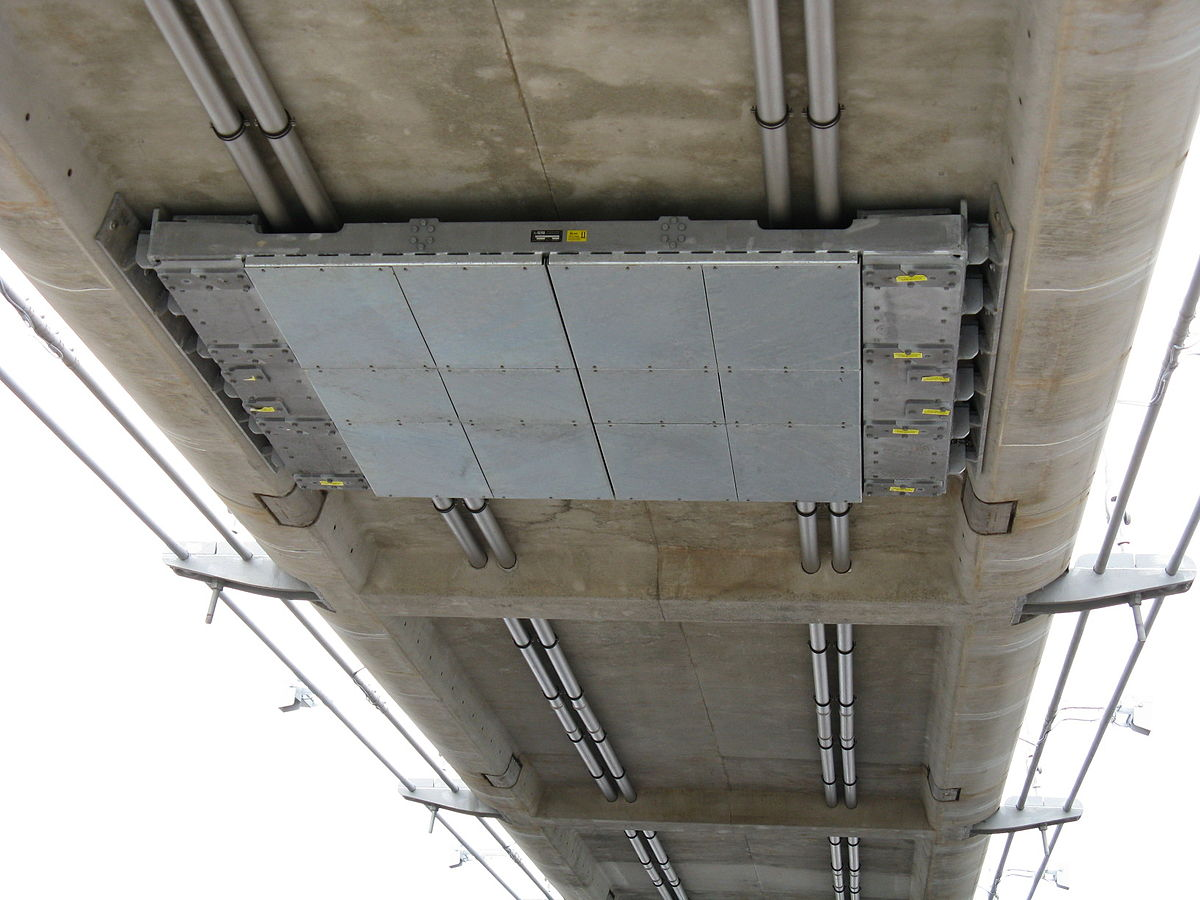
\includegraphics[width=\textwidth]{Image/TMD pont.jpg}
					\caption{Tuned mass damper sur l'Infinity bridge}
				\end{figure}
				
			\end{column}
			\begin{column}{0.45\textwidth}
				\begin{figure}
					\centering
					\caption{ Pendule de la tour Tapei 101 à Taiwan}
					\includegraphics[width=\textwidth]{Image/Taipeï.jpg}
				\end{figure}
			\end{column}
		\end{columns}
		\bigskip\small TMD = Tuned mass damper
	\end{frame}
	
	%\section{First section}
	\begin{frame}{Préambule}
		\frametitle{Objectifs}
		\underline{Problématique:} Quelle est l'influence du TMD sur la stabilité de la tour ? 
		\vspace{12pt}
		\linebreak[3]Objectifs du TIPE:
		\begin{itemize}
			\item Maquettiser un immeuble
			\item Élaborer une excitation sinusoïdale de fréquence paramétrable
			\item Mesurer la position relative de l'immeuble
			
		\end{itemize}
		
	\end{frame}
	
	\begin{frame}{Plan}
		\begin{enumerate}
			\item Modèle théorique
			\item Maquettisation de l'immeuble
			\item Création de l'axe d'excitation
			\item Élaboration de l'ensemble des capteurs
		\end{enumerate}
	\end{frame}
	\section{Théorie}
	\begin{frame}
		\begin{columns}
			\begin{column}{0.5\textwidth}
				\begin{figure}
					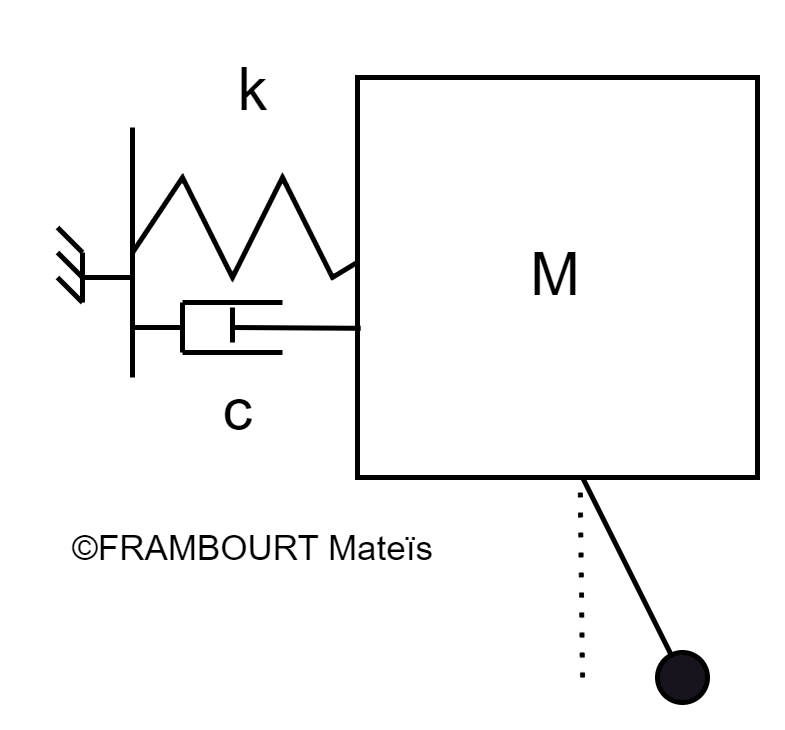
\includegraphics[width=\textwidth]{Image/Schéma modélisation.png}
					\caption{Schéma de la modélisation}
				\end{figure}
			\end{column}
			\begin{column}{0.5\textwidth}
				PDF à la masse : 
				$M\ddot{x} = -kx -c\dot{x} + f(t)$\\
				On a donc sans le pendule : $H=\frac{1}{1+j\frac{c}{k}\omega-\frac{M}{k}\omega^2}$ 
				
			\end{column}
		\end{columns}
	\end{frame}
	\begin{frame}{Élaboration d'un modèle théorique}
		\frametitle{Modélisation du système avec pendule}
		Oscillations linéaires , on peut modéliser le pendule par un système masse ressort
		\begin{columns}
			\begin{column}{0.5\textwidth}
				\begin{figure}
					\centering
					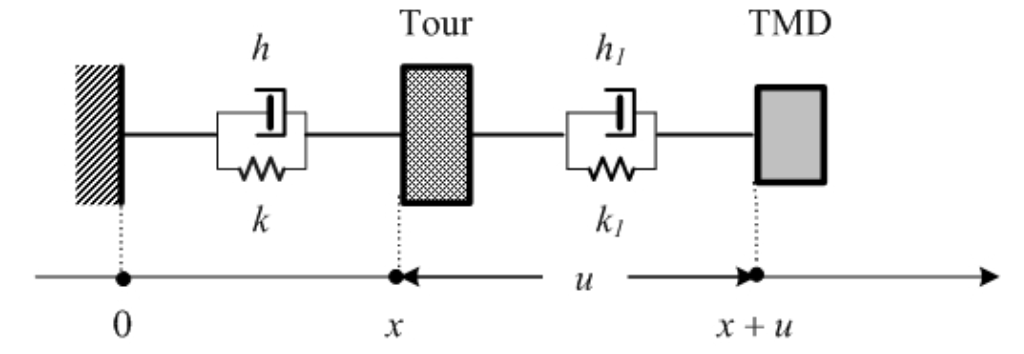
\includegraphics[width=1\textwidth]{Image Noé/ModelisationMP.png}
					\caption{Modèle équivalent du système}
				\end{figure}
			\end{column}
			\begin{column}{0.5\textwidth}
				\begin{itemize}
					\item m=Masse du pendule
					\item M=Masse de la tour
					\item $k_{1}$=Coefficient de raideur élastique du pendule
					\item k=Coefficient de raideur élastique (Baguettes + bouchons dans notre modèle)
					\item $h_{1}$= coefficient de frottement du pendule 
					\item h=coefficient de frottement de la tour
				\end{itemize}	
			\end{column}
		\end{columns}
		
	\end{frame}


	\begin{frame}{Équations du système}
		L'excitation extérieure est modélisée par une force $f_{0}(t)$ appliquée à la tour\vspace{12pt}
		PFD à ${tour + TMD}$:
		\begin{equation}\label{key}
			M\ddot{x} + m(\ddot{x}+\ddot{u}) +h\dot{x} + kx = f_{0}(t)
		\end{equation}\\
		\vspace{12pt}
		PFD  au TMD uniquement:
		\begin{equation}
			m(\ddot{x}+\ddot{u}) + h_{1}\dot{u} + k_{1}u = 0
		\end{equation}\\
	
		
	\end{frame}
	
	\begin{frame}{Fonctions de transfert du système}
		
	\begin{empheq}[left=\empheqlbrace]{align*}
		H1(\omega)&=\frac{U}{X}= \frac{m\omega^{2}}{k_{1}+jh_{1}\omega-m\omega^{2}}\\
		H2(\omega)&=\frac{X}{\frac{F_{0}}{k}}= \frac{1}{1+j\frac{h}{k}\omega-\frac{(M+m)}{k}\omega^2-\frac{H1(\omega)}{k}\omega^2}
	\end{empheq}
	\vspace{12 pt}
	
	H2 représente le rapport de l'amplitude de l'accélération ressentie par les occupants de  la tour et de l'amplitude de l'accélération extérieure que subit la tour
	
	
		
		
	\end{frame}
	\section{Maquette} 
	\begin{frame}{Objectif de la Maquettisation}
		\begin{columns}
		\begin{column}{0.3\textwidth}
			
		
		
		\begin{itemize}
			\item Objectif : Obtenir un comportement similaire 
			\item étude de différente solution
		\end{itemize}
	\end{column}
	\begin{column}{0.7\textwidth}
		\begin{figure}
			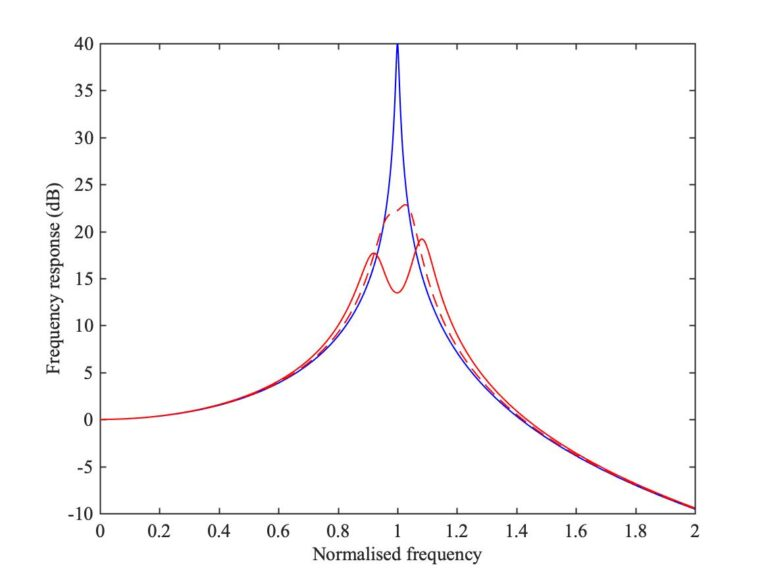
\includegraphics[width=\textwidth]{Image/Objectif en courbe.jpg}
			\caption{\copyright euphonics.org}
		\end{figure}
	\end{column}
	\end{columns}
	\end{frame}
	\begin{frame}{modèle naïf}
		\begin{columns}
			\begin{column}{0.25\textwidth}
			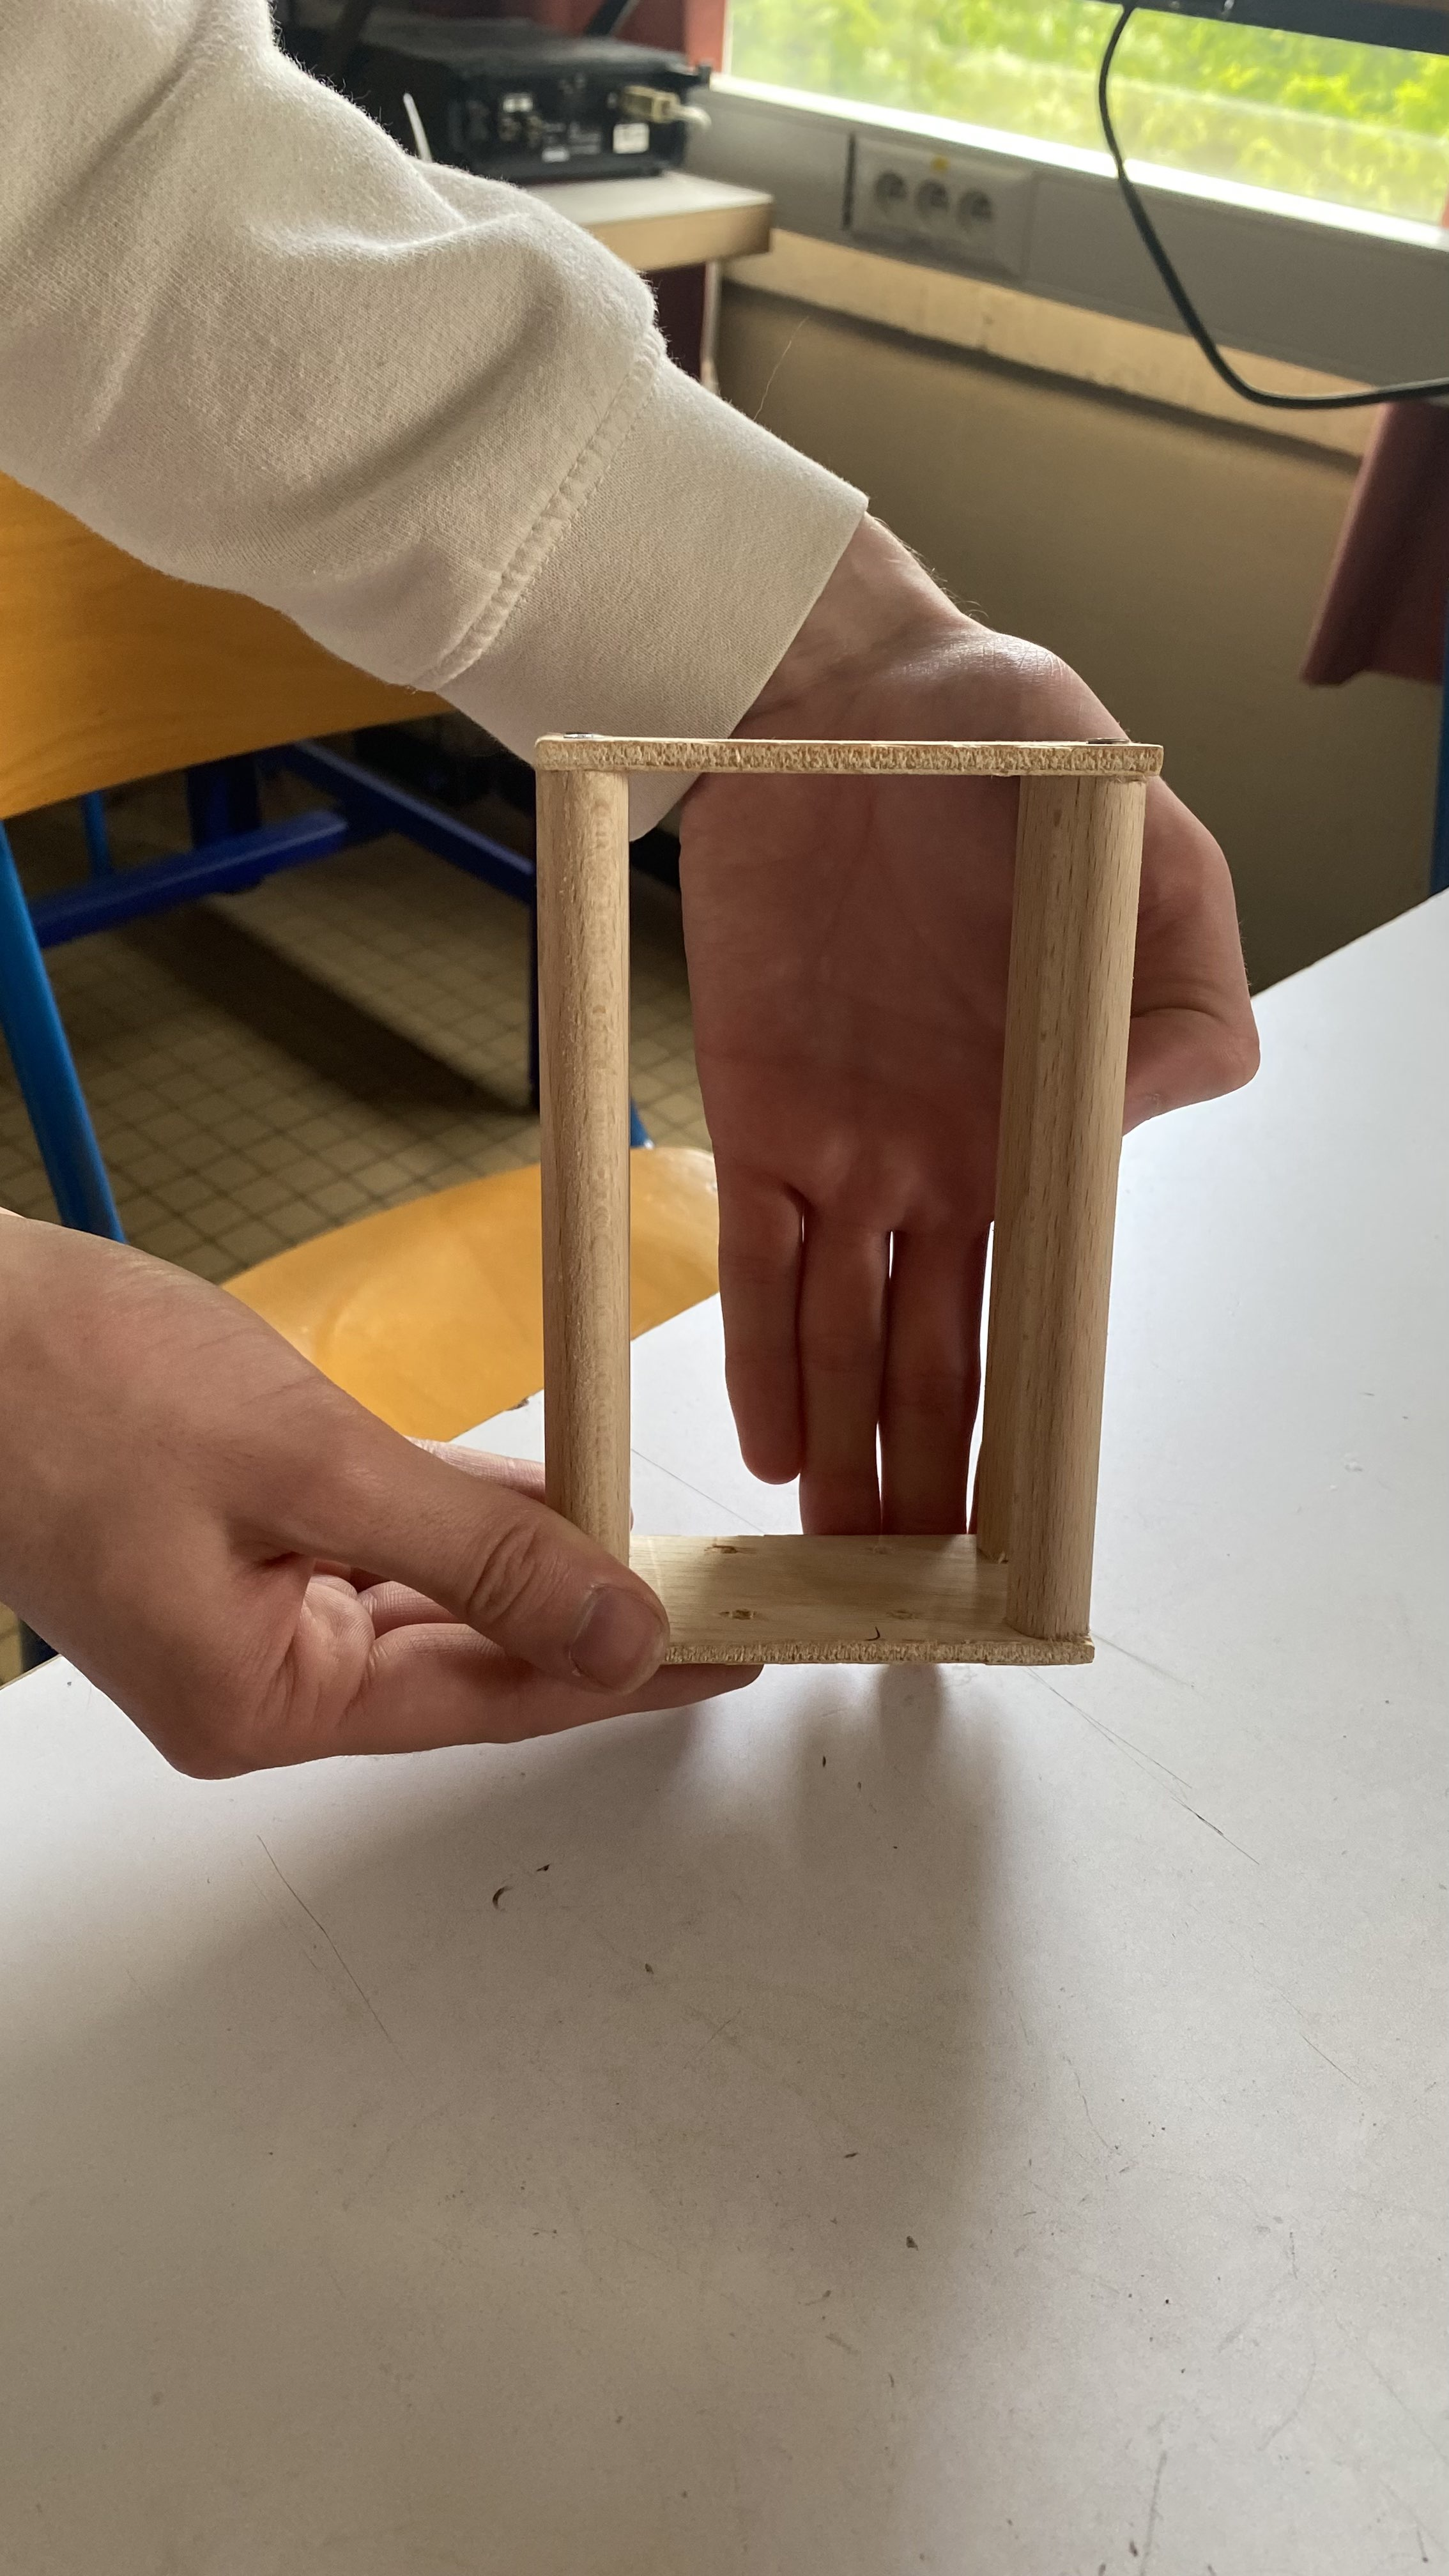
\includegraphics[width=\textwidth]{Image/Modèle solide face échelle main.jpg}
			
		\end{column}
		\begin{column}{0.25\textwidth}
		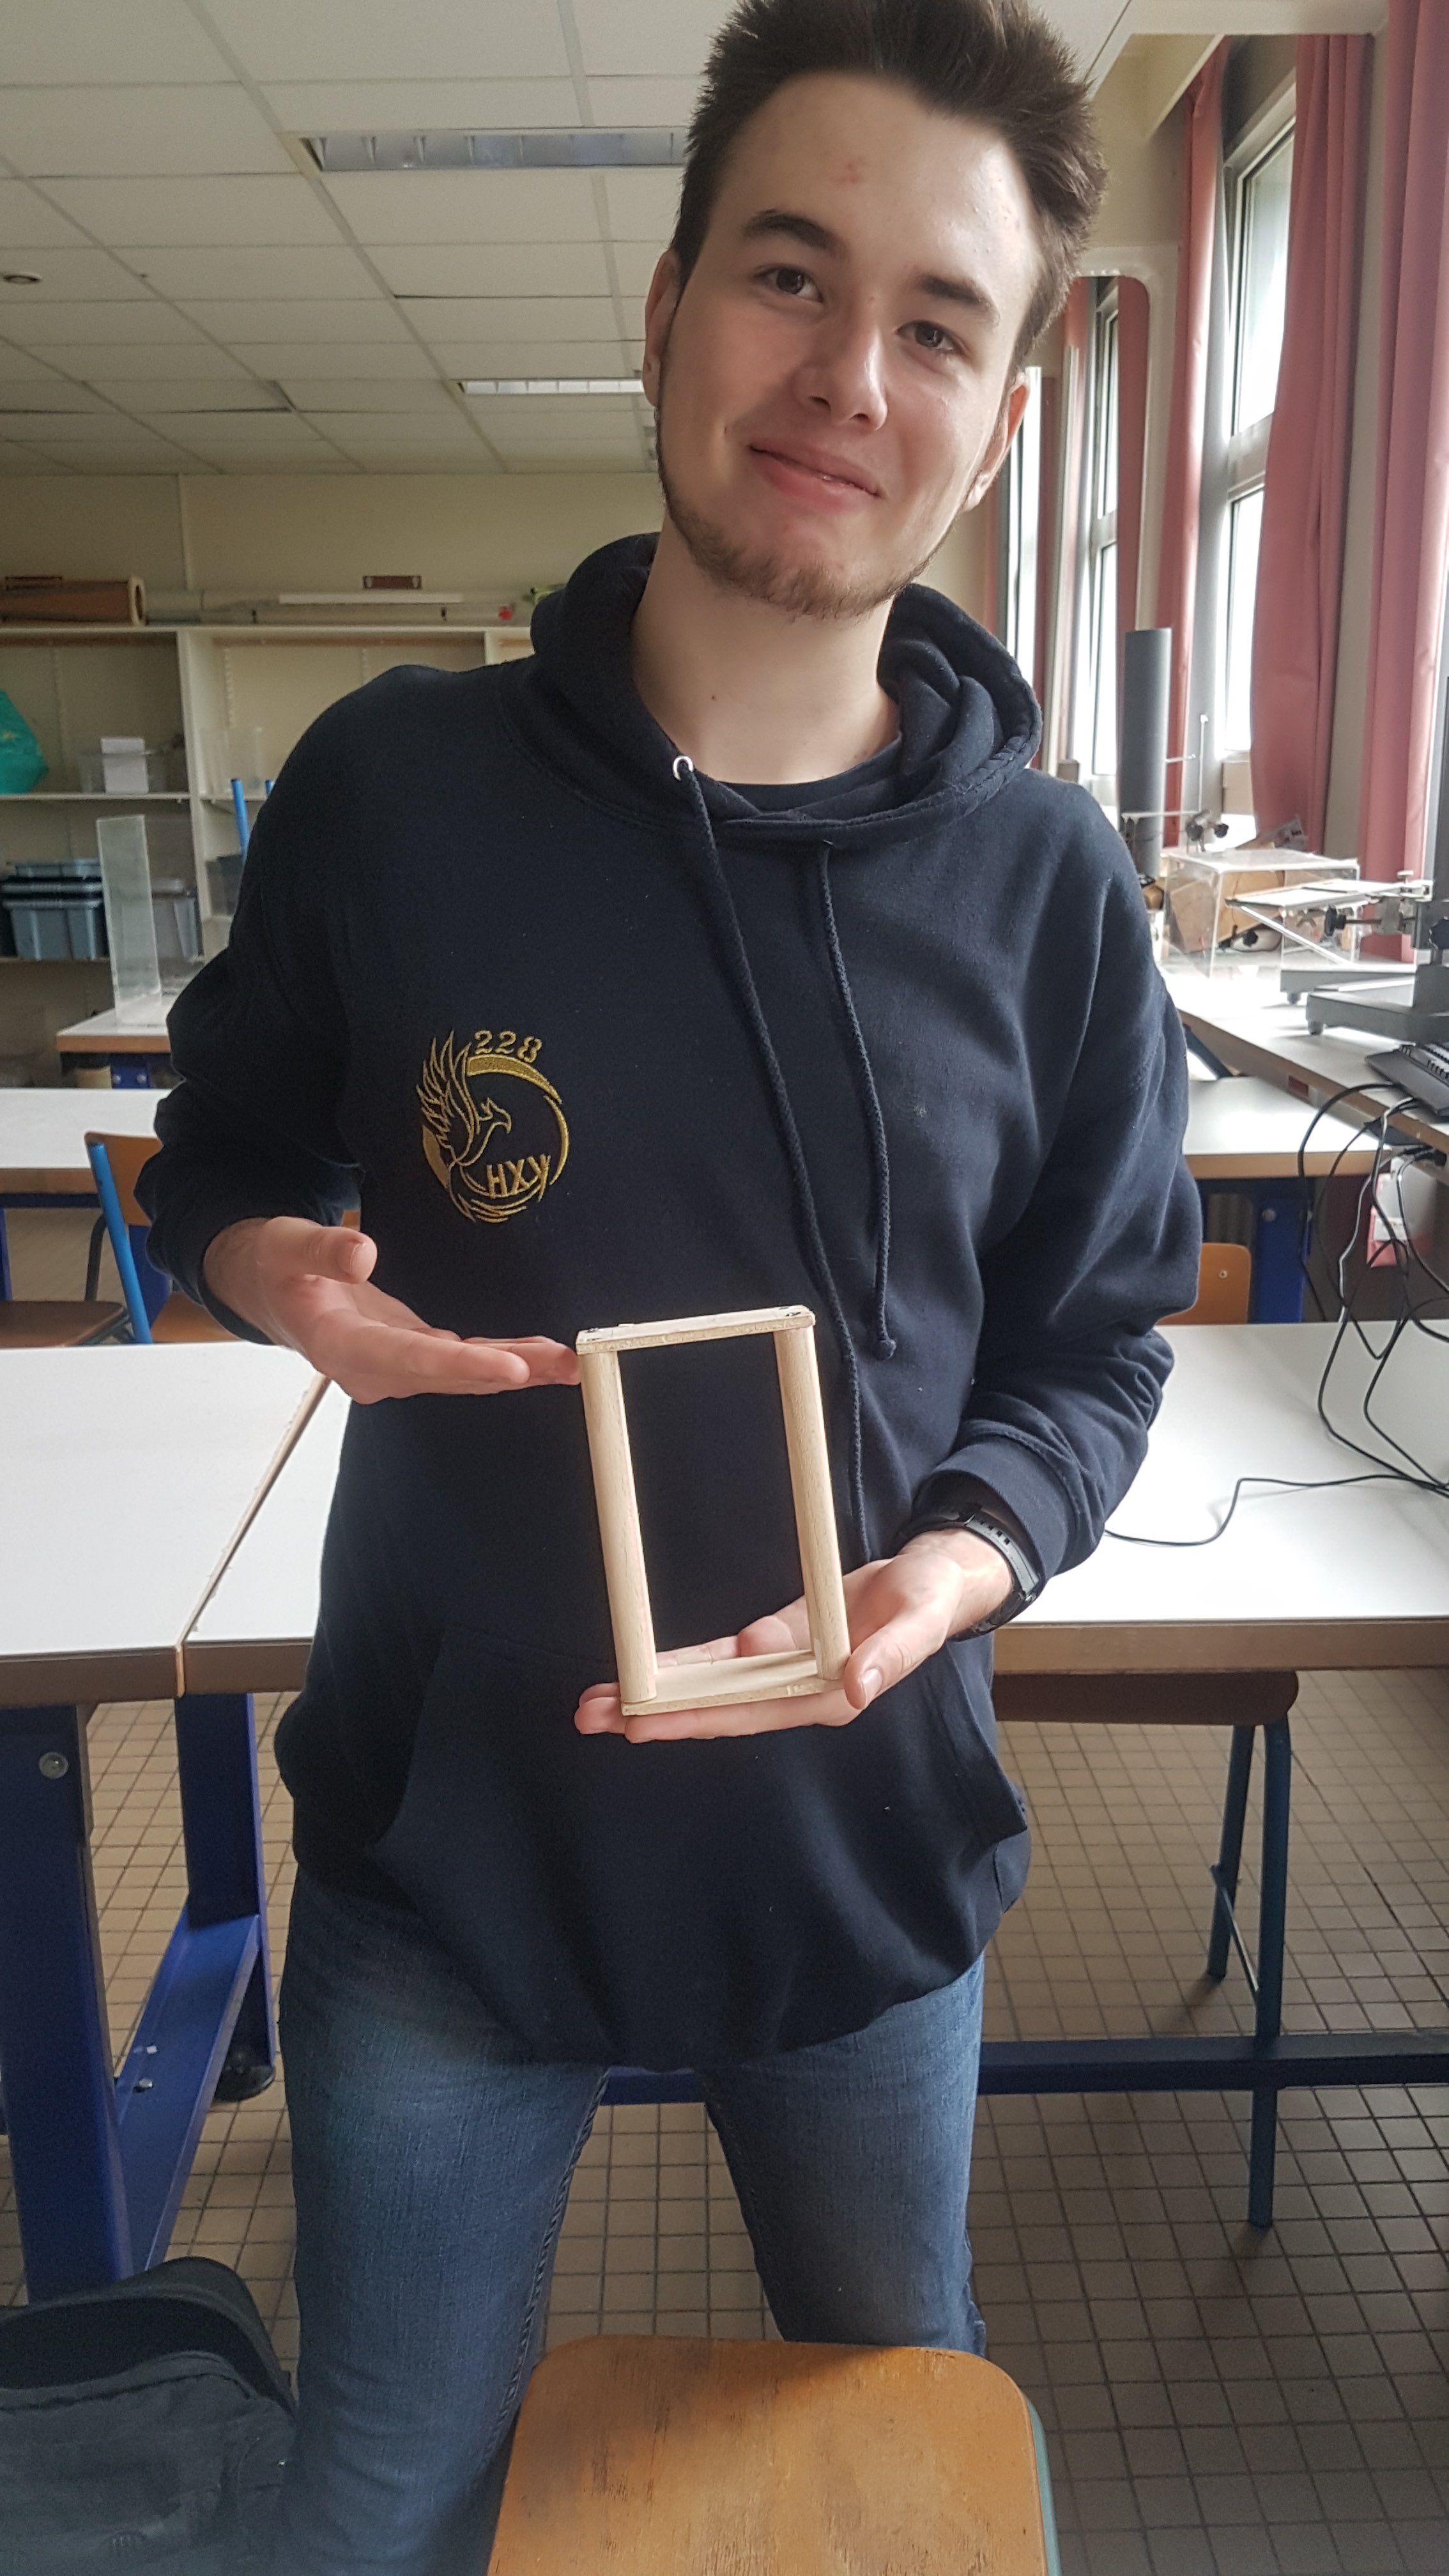
\includegraphics[width=\textwidth]{Image/Photo Mateïs échelle modèle solide.jpg}
			
		\end{column}
		\begin{column}{0.25\textwidth}
		\includegraphics[width=\textwidth]{Image/Modèle solide Profil.jpg}
		
		\end{column}
		\begin{column}{0.25\textwidth}
			\begin{itemize}
				\item Rapide à construire 
				\item trop rigide
			\end{itemize}
		\end{column}
		\end{columns}
		
	\end{frame}
\begin{frame}{Modèle flexible}
	\begin{columns}
		\begin{column}{0.25\textwidth}
			\begin{figure}
				
			
			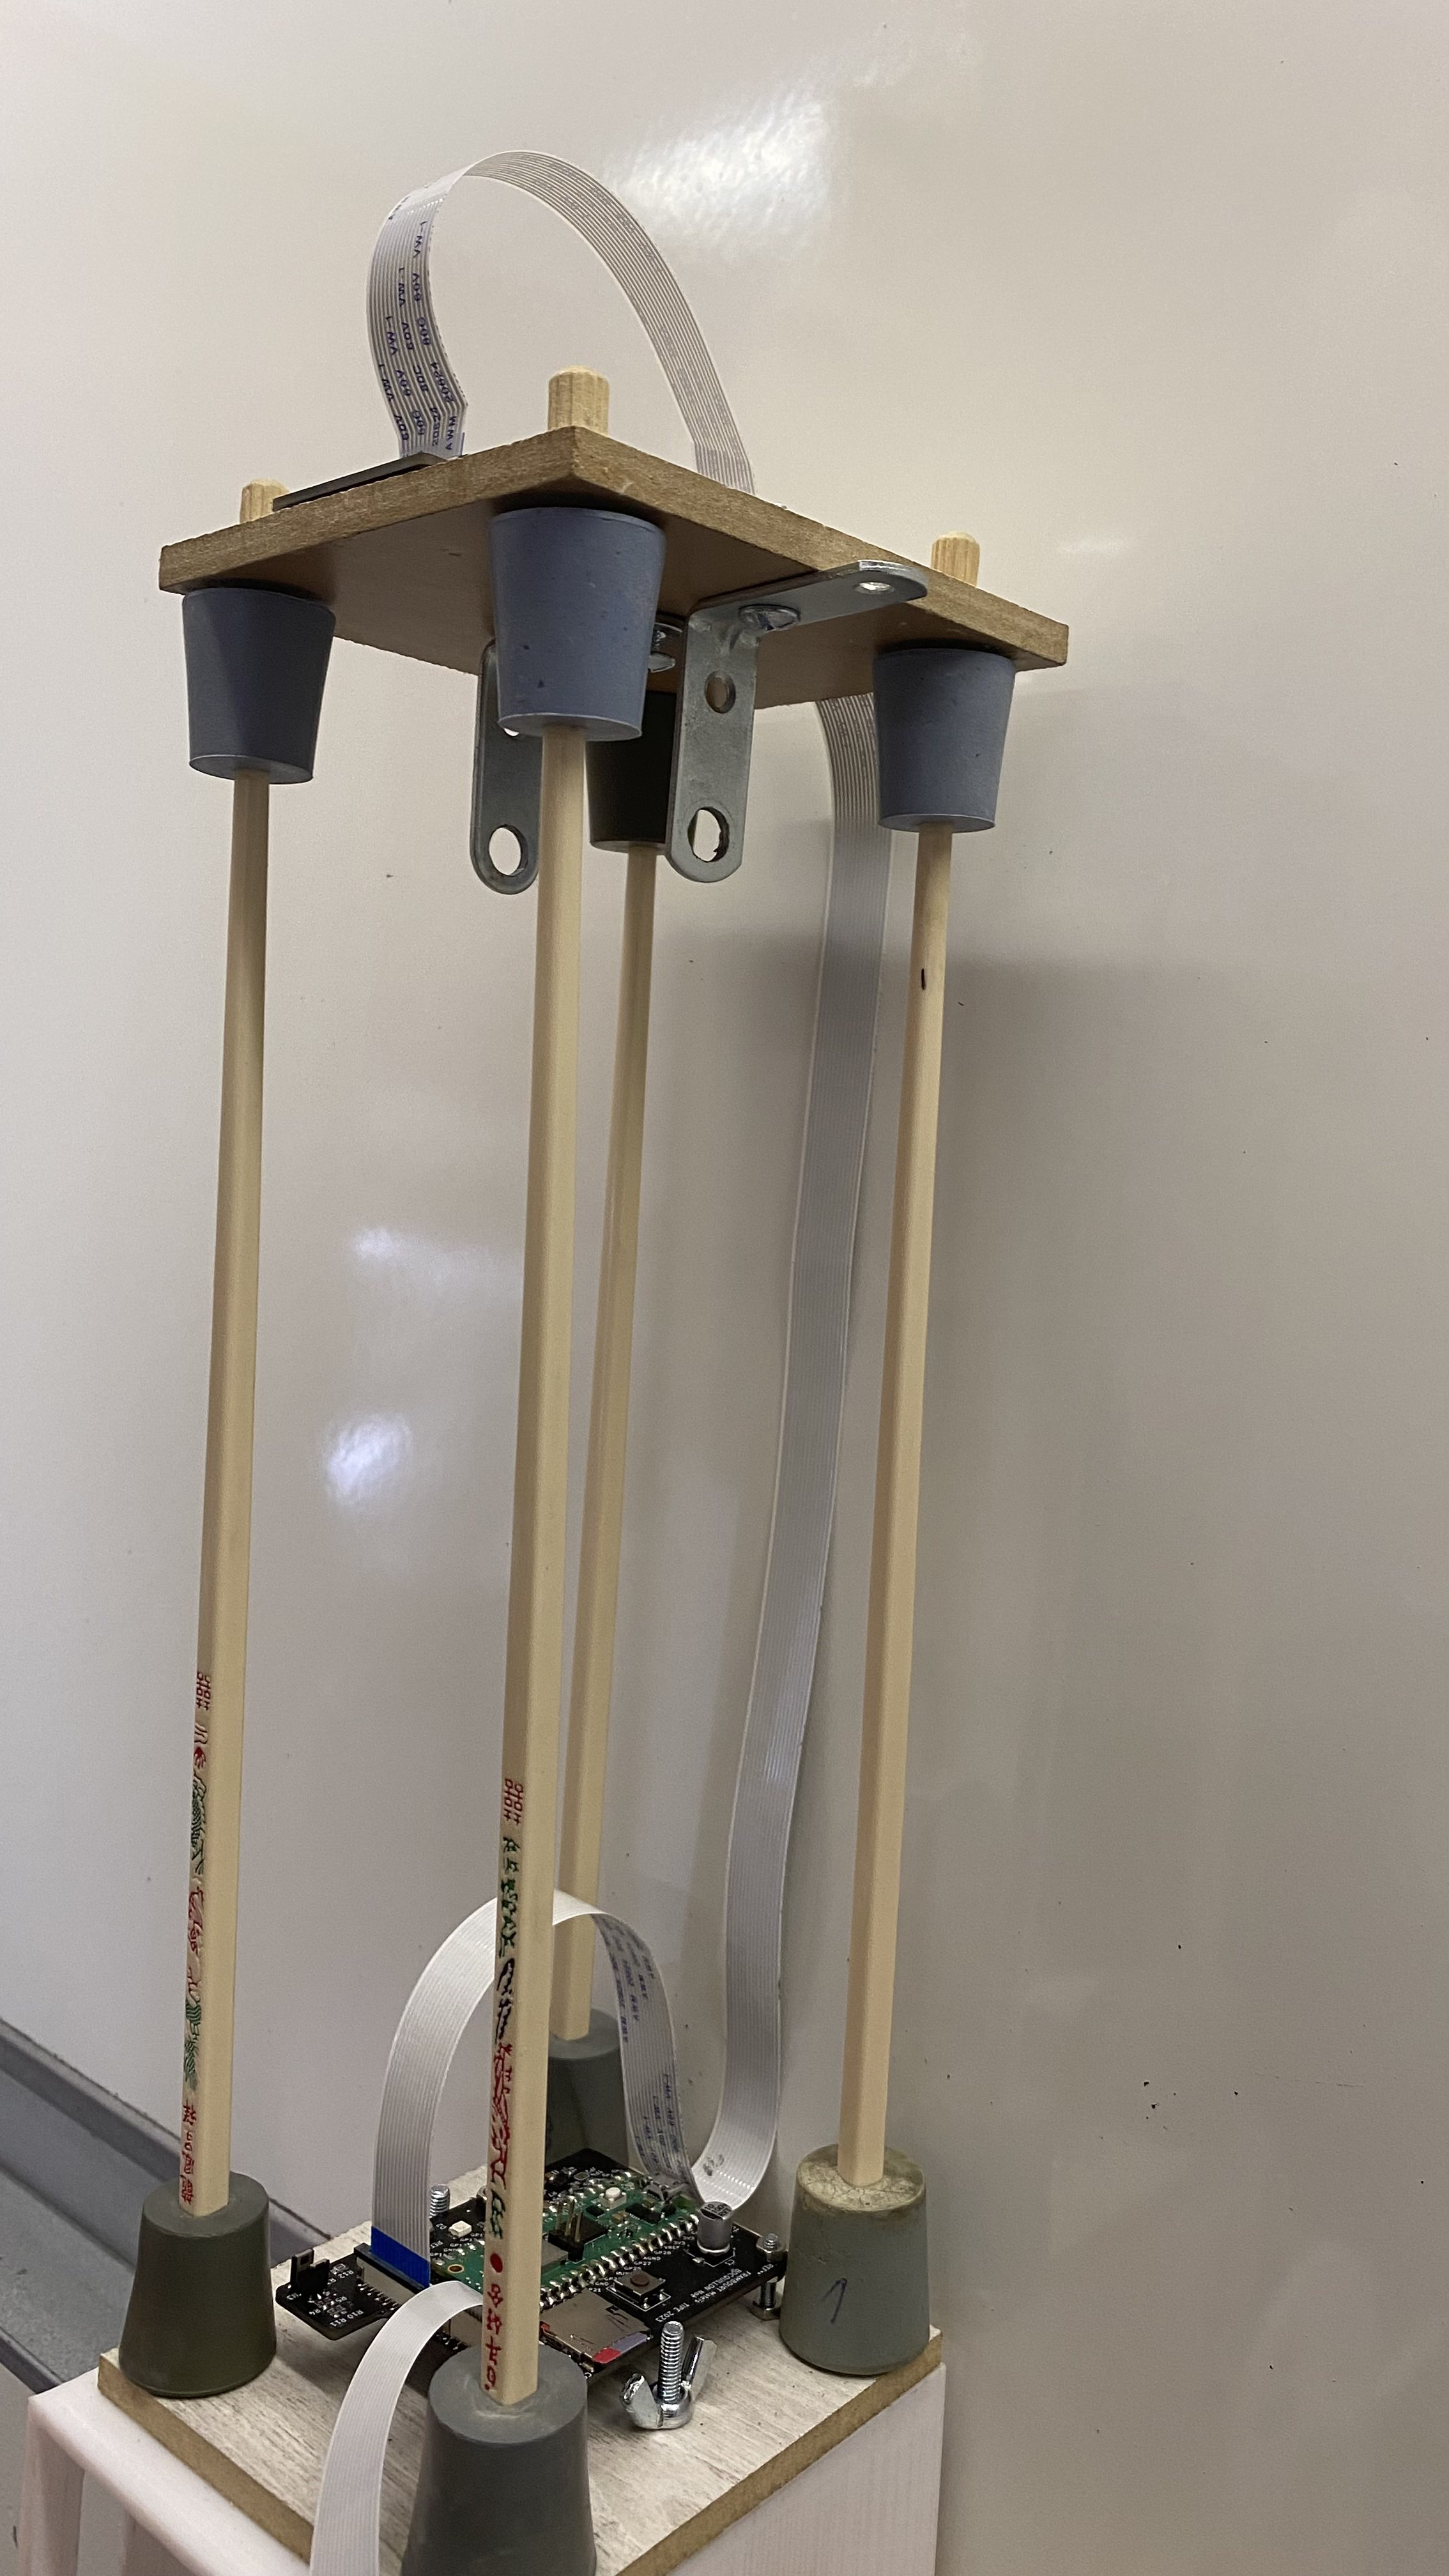
\includegraphics[width=\textwidth]{Image/Tour flexible sur tableau blanc.jpg}
			\caption{Tour flexible}
		\end{figure}
		\end{column}
		\begin{column}{0.75\textwidth}
			\begin{figure}
				
			
		\includegraphics[width=\textwidth]{Image/modèle incorrect.png}
		\caption{Modèle incorrect mais allure bonne}
	\end{figure}	
		\end{column}
	\end{columns}
\end{frame}
\begin{frame}
	\begin{columns}
		\begin{column}{0.3\textwidth}
			
		
	
	Contrainte : 
	\begin{itemize}
		\item Fonctionnement linéaire 
		\item Résonance dans l'intervalle [0.5,7Hz]
		\item facilement modifiable
	\end{itemize}
\end{column}
\begin{column}{0.3\textwidth}
	Limite imposée : 
	\begin{itemize}
		\item faible amplitude d'oscillations
		\item surface minimale
	\end{itemize}

\end{column}
\begin{column}{0.3\textwidth}
	\begin{figure}
		\includegraphics[width=\textwidth]{Image/schéma global.png}
		\caption{Schéma global}
	\end{figure}
\end{column}
\end{columns}
\end{frame}
\begin{frame}{problème de non-linéarité}
	\begin{columns}
		\begin{column}{0.35\textwidth}
			\begin{figure}
				
			
			\includegraphics[width=\textwidth]{Image/Problème de torsion.jpg}
			\caption{Problème de torsion}
		\end{figure}
		\end{column}
		\begin{column}{0.35\textwidth}
			\begin{figure}
				\includegraphics[width=\textwidth]{Image/Cause de la torsion.jpg}
				\caption{Cause de la torsion}
			\end{figure}
		\end{column}
	\end{columns}
\end{frame}
\begin{frame}{Pendule réglable}
	\begin{columns}
		
	\begin{column}{0.35\textwidth}
		
	
	\begin{figure}
		\includegraphics[width=\textwidth]{Image/Pendule réglable 2.jpg}
		\caption{Pendule à tige filetée}
	\end{figure}
\end{column}
\begin{column}{0.65\textwidth}
	Contrainte : 
	\begin{itemize}
		\item Minimum de frottement
		\item Centre de gravité réglable
		\item masse réglable
	\end{itemize}
\end{column}
\end{columns}
\end{frame}
\section{Mise en vibration de la maquette}

	
	\begin{frame}{Guidage}
		\frametitle{Premier guidage}
 
		\begin{columns}
			\begin{column}{0.5\textwidth}
				\begin{figure}
					\includegraphics[width=\textwidth]{Image/Axe de l'ancien TIPE.jpg}
					\caption{Guidage récupéré d'un ancien TIPE}
				\end{figure}
			\end{column}
			\begin{column}{0.5\textwidth}
				Avantages:
				\begin{itemize}
					\item Déjà construit
				\end{itemize}
				\vspace{12pt}
				Inconvénients:
				
				\begin{itemize}
					\item Hystérésis
					\item Frottement non négligeable
					\item Asservissement à réaliser
				\end{itemize}
			\end{column}
		\end{columns}
	\end{frame}
	\begin{frame}{Guidage récupéré}
		\begin{columns}[T]
			\begin{column}{0.8\textwidth}
				\begin{figure}
					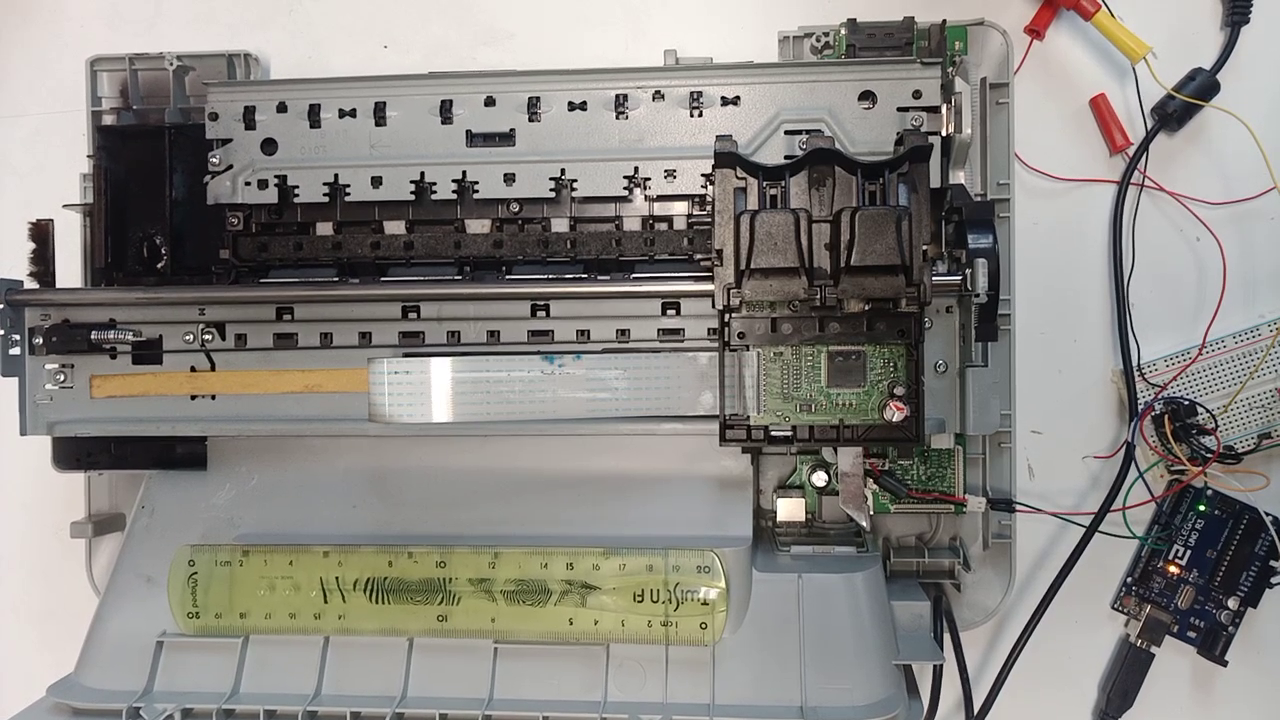
\includegraphics[width=\textwidth]{Image/Imprimante.png}
					\caption{Axe d'une imprimante jets d'encre}
				\end{figure}
			\end{column}
		\end{columns}
	\end{frame}
		\begin{frame}
			\begin{columns}
				\begin{column}{0.5\textwidth} 
				\begin{figure}
					\includegraphics[width=\textwidth]{Image/oscillation début.png}
					\caption{début des oscillations}
				\end{figure}
				
				
			\end{column}
			\begin{column}{0.5\textwidth} 
				\begin{figure}
					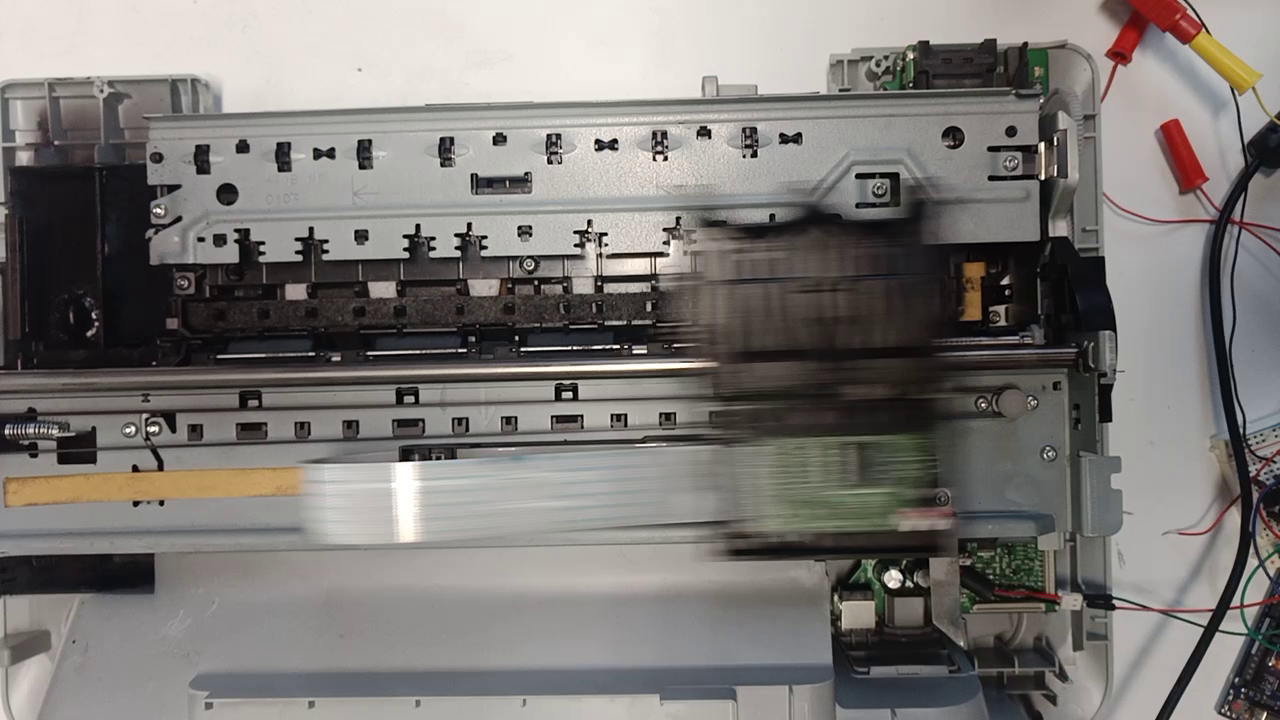
\includegraphics[width=\textwidth]{Image/oscillation fin.png}
					\caption{fin des oscillations}
				\end{figure}
				
			\end{column}
		\end{columns}
	\end{frame}
	\begin{frame}{solution à ces problème}
		\begin{columns}
			\begin{column}{0.3\textwidth}
				\begin{figure}
					\includegraphics[width=\textwidth]{Image/Solution au décalage.png}
					\caption{Solution au décalage}
				\end{figure}
			\end{column}
			\begin{column}{0.3\textwidth}
				\begin{figure}
					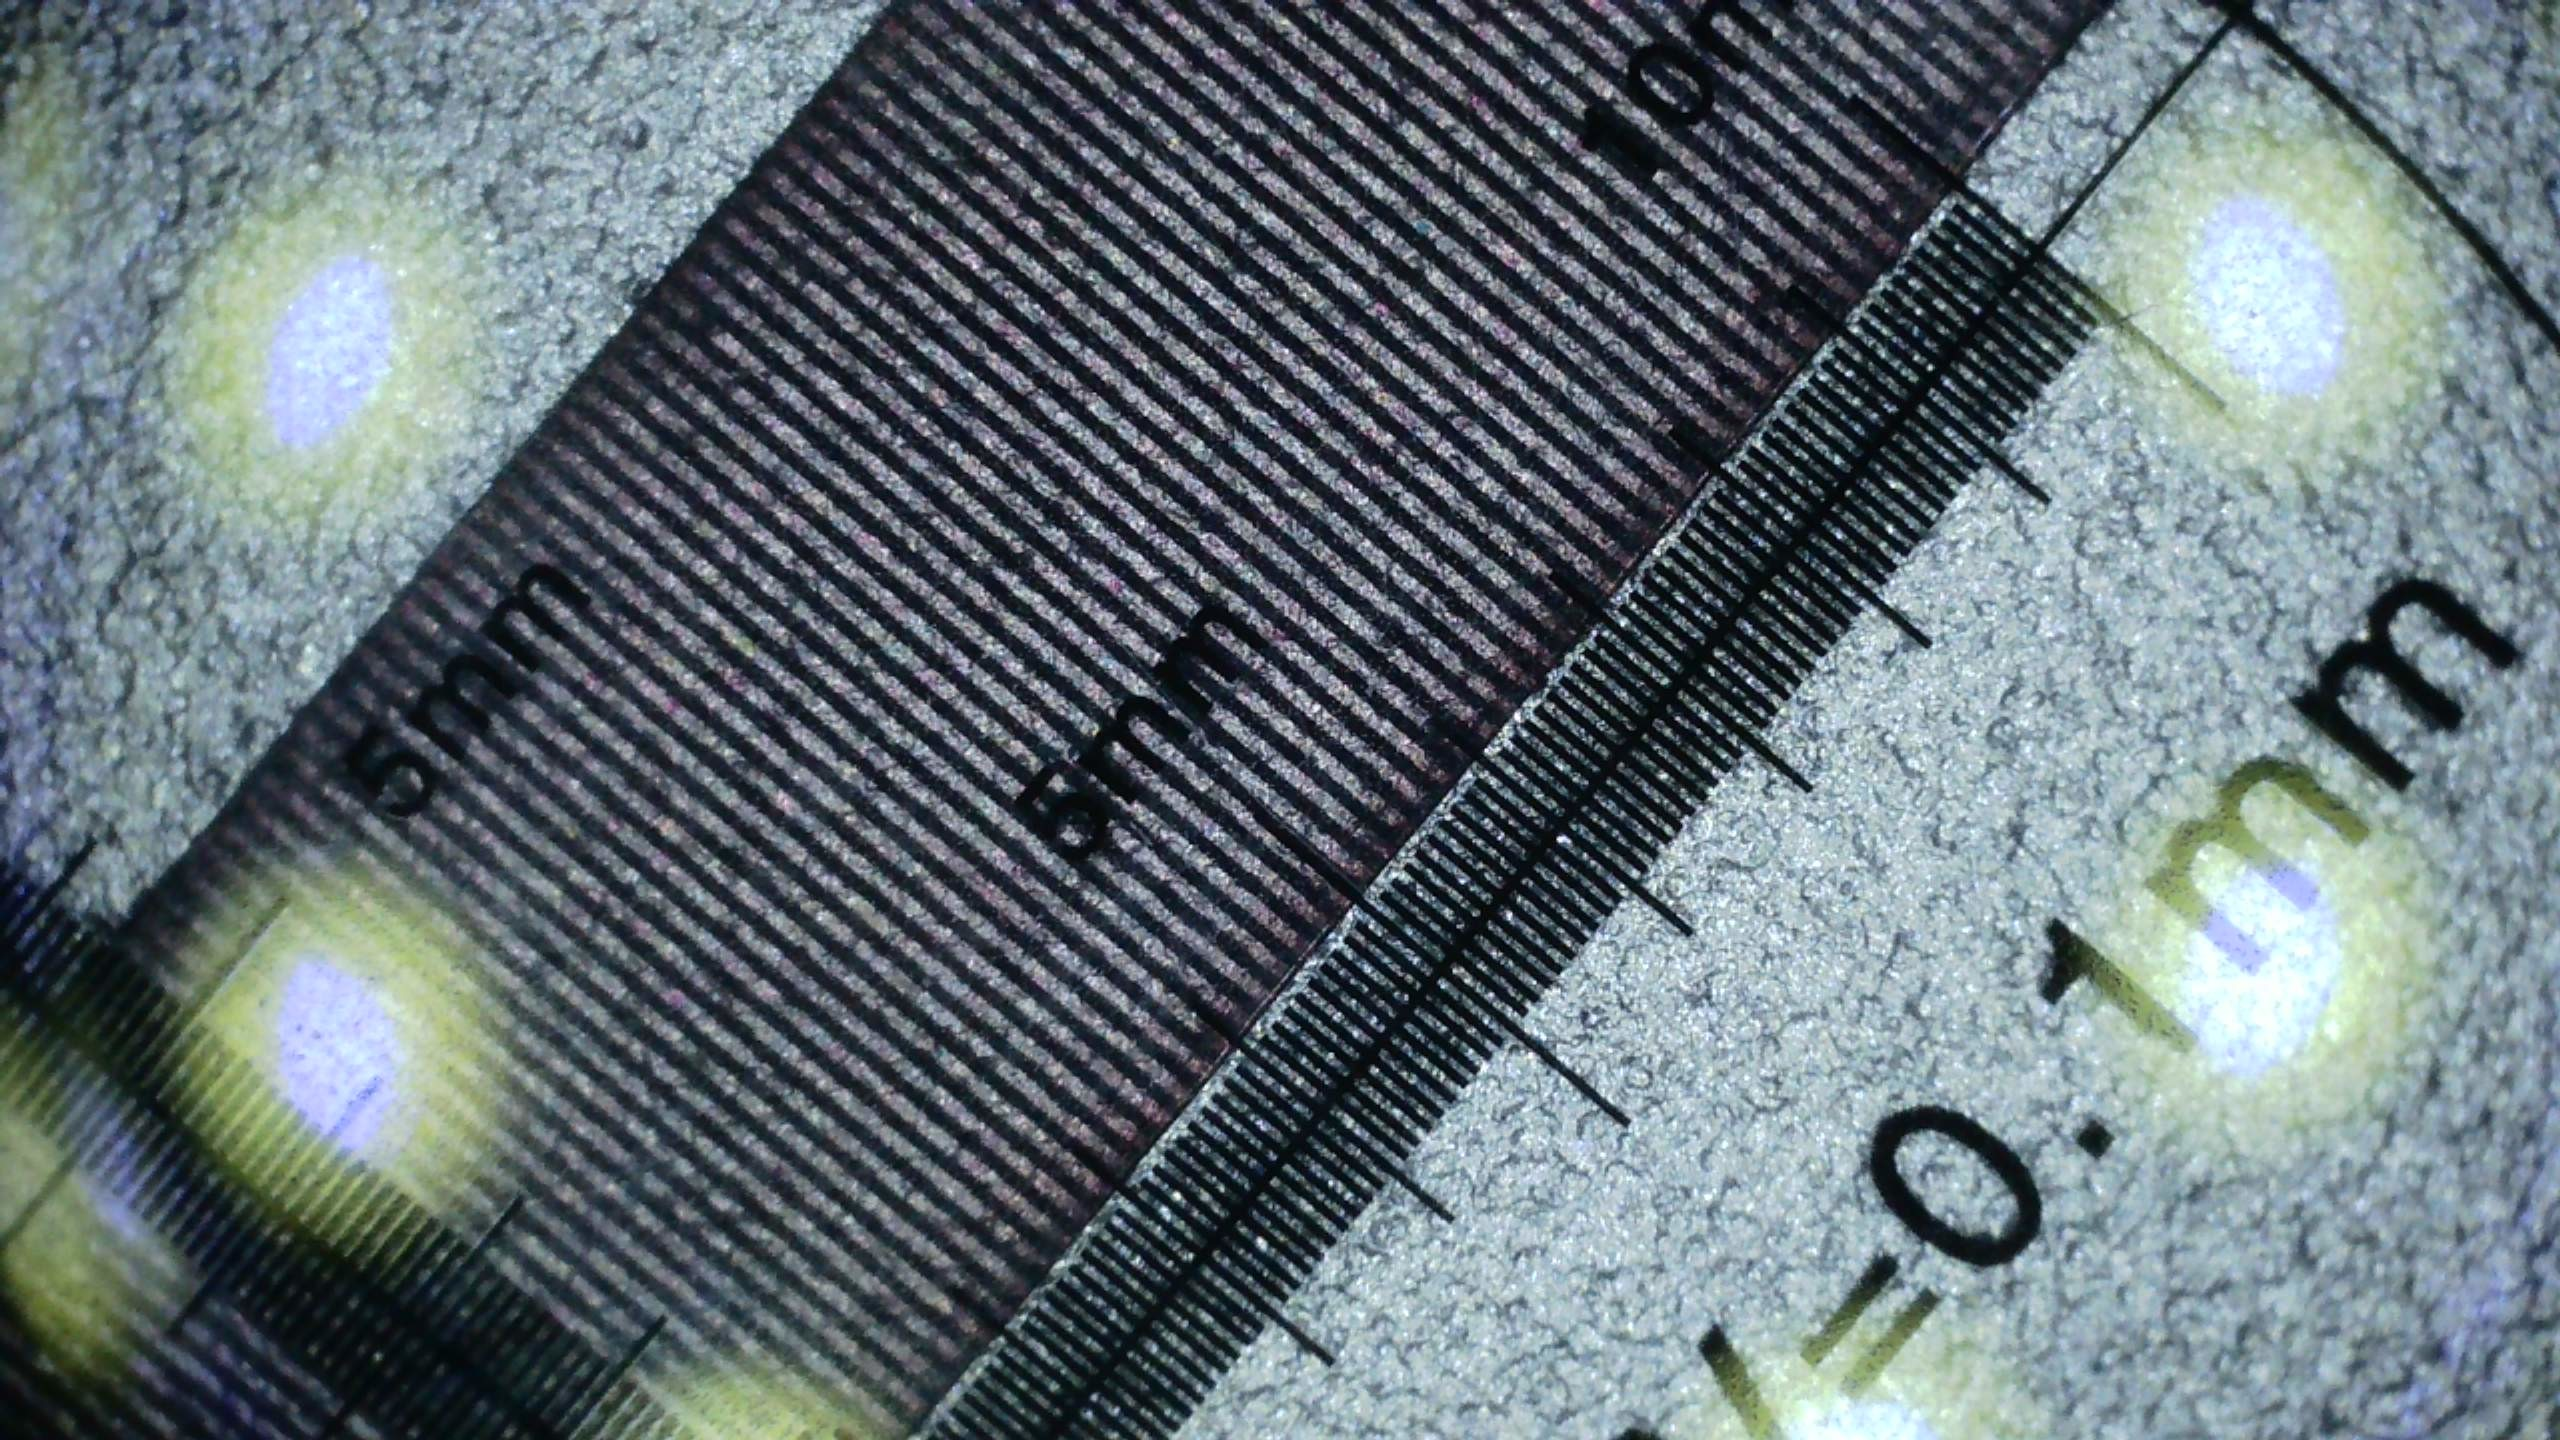
\includegraphics[width=\textwidth]{Image/Mesure ruban imprimante.jpg}
					\caption{Mesure du ruban zébré de l'imprimante}
				\end{figure}
				$d=0.2\pm0.05mm$
			\end{column}
			\begin{column}{0.3\textwidth}
				\begin{figure}

					\includegraphics[width=\textwidth]{Image/Soudure Carte imprimante récupérée.jpg}
					\caption{Tentative de récupération du capteur}
				\end{figure}
			\end{column}
		\end{columns}
		
	\end{frame}
	\begin{frame}{Conclusion sur cet axe}
		\begin{columns}
			\begin{column}{0.5\textwidth}
				Avantages : 
				\begin{itemize}
					\item Gratuit
					\item Solution mécanique déjà construite
				\end{itemize}
			\end{column}
			\begin{column}{0.5\textwidth}
				Inconvénients : 
				\begin{itemize}
					\item Asservissement à réaliser
					\item Dépendance entre la charge et le déplacement
					\item Moteur faible
				\end{itemize}
			\end{column}
		\end{columns}
	\end{frame}
\begin{frame}{Axe imprimé en 3D}
	\begin{columns}
		\begin{column}{0.5\textwidth}
			\begin{figure}
				\includegraphics[width=\textwidth]{Image/Schéma oscillateur position droite.drawio.png}
				\caption{Schéma cinématique de l'axe}
			\end{figure}
		\end{column}
		\begin{column}{0.5\textwidth}
			\begin{figure}
				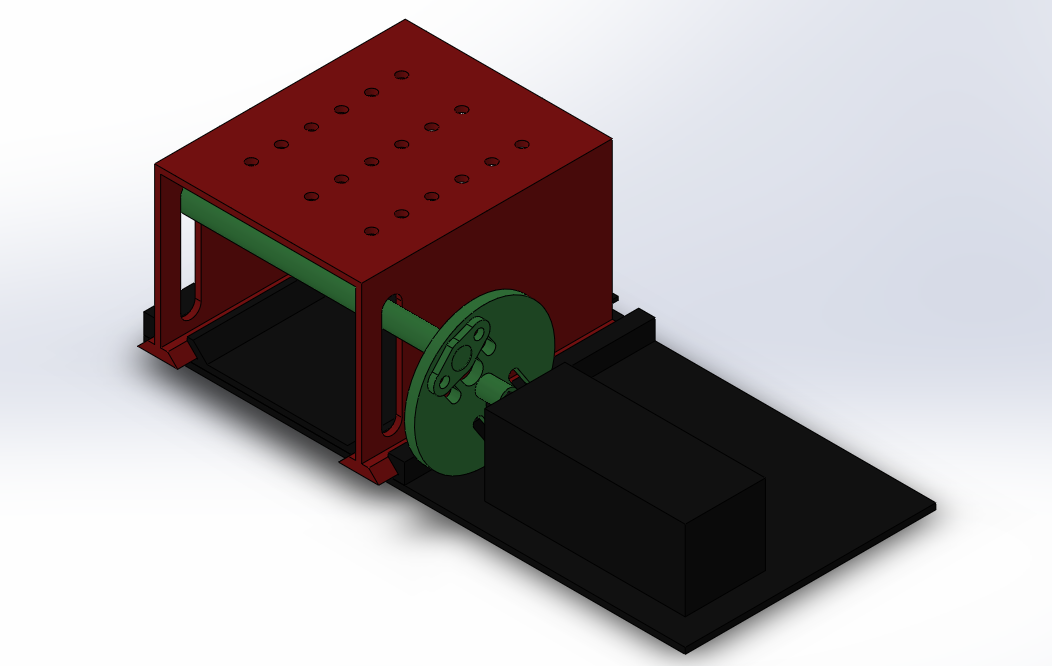
\includegraphics[width=\textwidth]{Image/montage excentrique.png}
				\caption{Montage sur Solidwork}
			\end{figure}
		\end{column}
	\end{columns}
\end{frame}
\begin{frame}{Hystérésis}
	\begin{columns}
		\begin{column}{0.5\textwidth}
			\begin{figure}
				\includegraphics[width=\textwidth]{Image/Schéma oscillateur position droite.drawio.png}
				\caption{Schéma cinématique de l'axe à droite}
			\end{figure}
		\end{column}
		\begin{column}{0.5\textwidth}
			\begin{figure}
				\includegraphics[width=\textwidth]{Image/Schéma oscillateur position gauche.png}
				\caption{Schéma à gauche}
			\end{figure}
		\end{column}
	\end{columns}
\end{frame}
\begin{frame}{Conclusion sur cet axe}
	\begin{columns}
		\begin{column}{0.3\textwidth}
			Avantages : 
			\begin{itemize}
				\item Modulaire
				\item Précise sans Asservissement
				\item facilement rêglable en fréquence
			\end{itemize}
		\end{column}
		\begin{column}{0.3\textwidth}
			Inconvénients : 
			\begin{itemize}
				\item Pièce fragile à l'usure
				\item Plateforme limité en taille
				\item Hystérésis
			\end{itemize}
			
		\end{column}
		\begin{column}{0.3\textwidth}
			\begin{figure}
				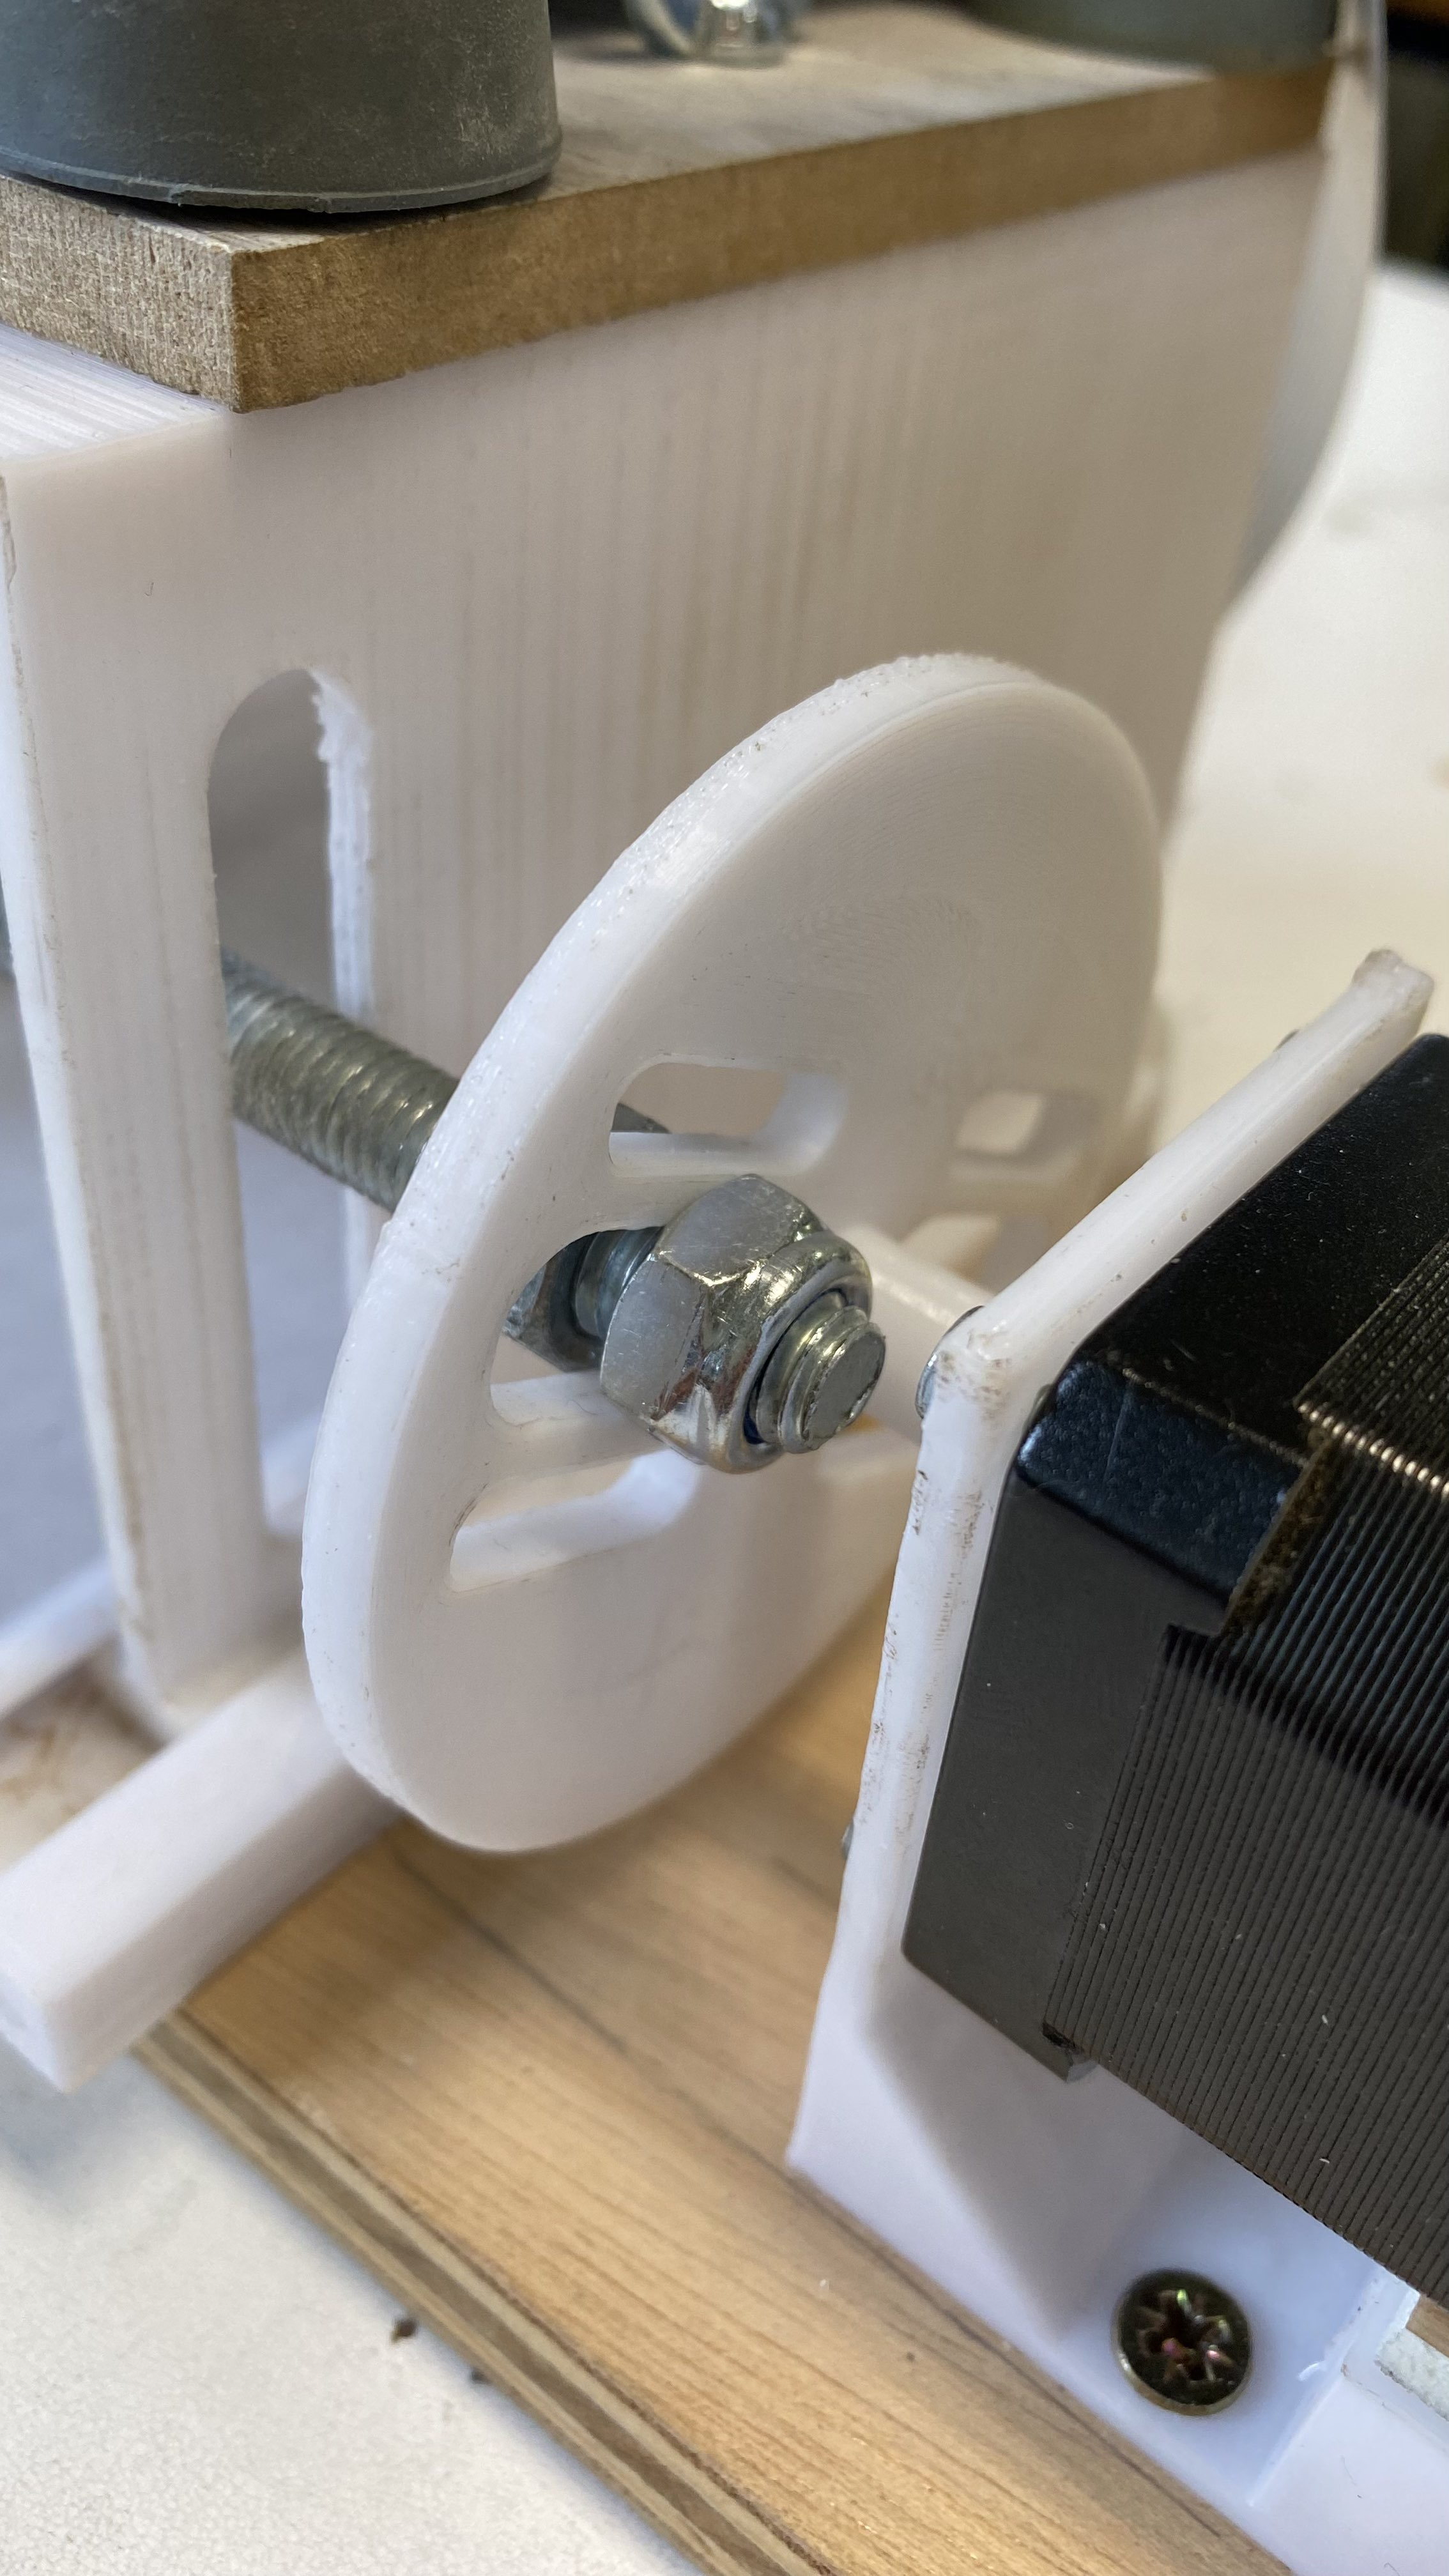
\includegraphics[width=\textwidth]{Image/Excentrique.jpg}
				\caption{Réalisation pratique}
			\end{figure}
		\end{column}
	\end{columns}
\end{frame}
	\begin{frame}{Capteurs}
		
		%schéma de la maquette avec des 2 accéléromètres
		
		\begin{columns}
			\begin{column}{0.35\textwidth}
				\begin{figure}
					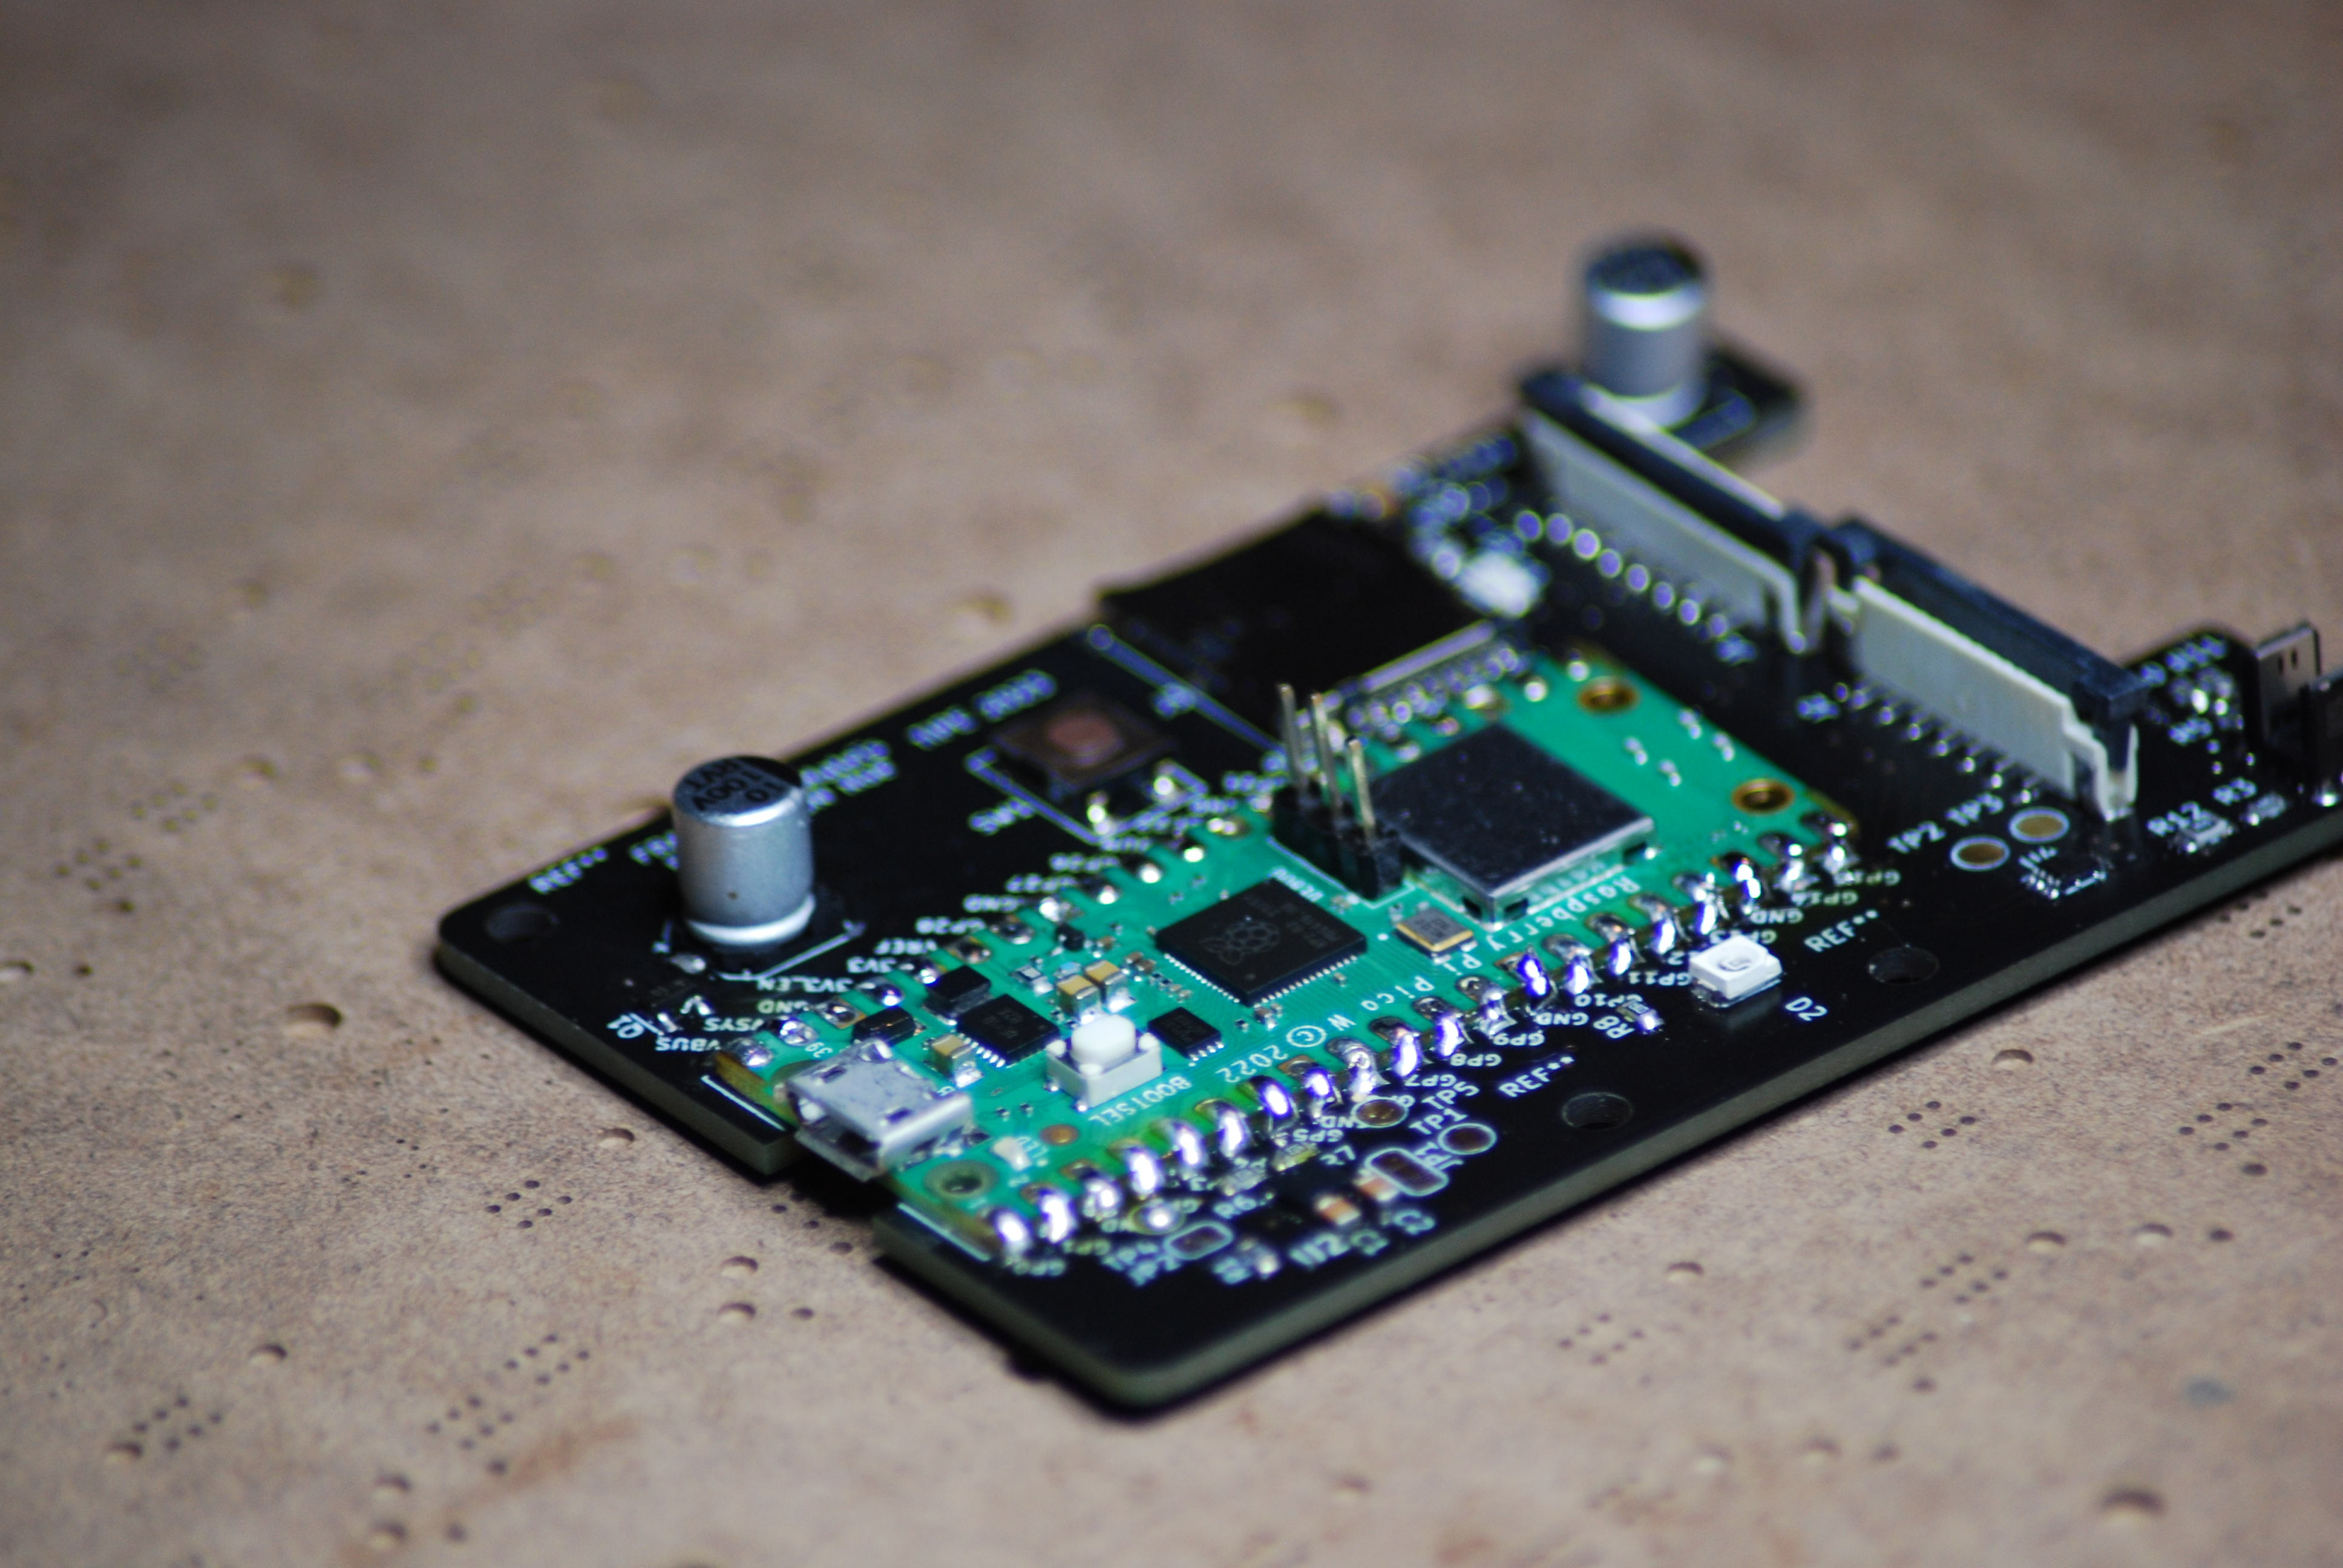
\includegraphics[width=\textwidth]{Image/Carte principale belle photo.JPG}
					\caption{Accéléromètre du socle}
				\end{figure}
			\end{column}
			\begin{column}{0.35\textwidth}
				\begin{figure}
					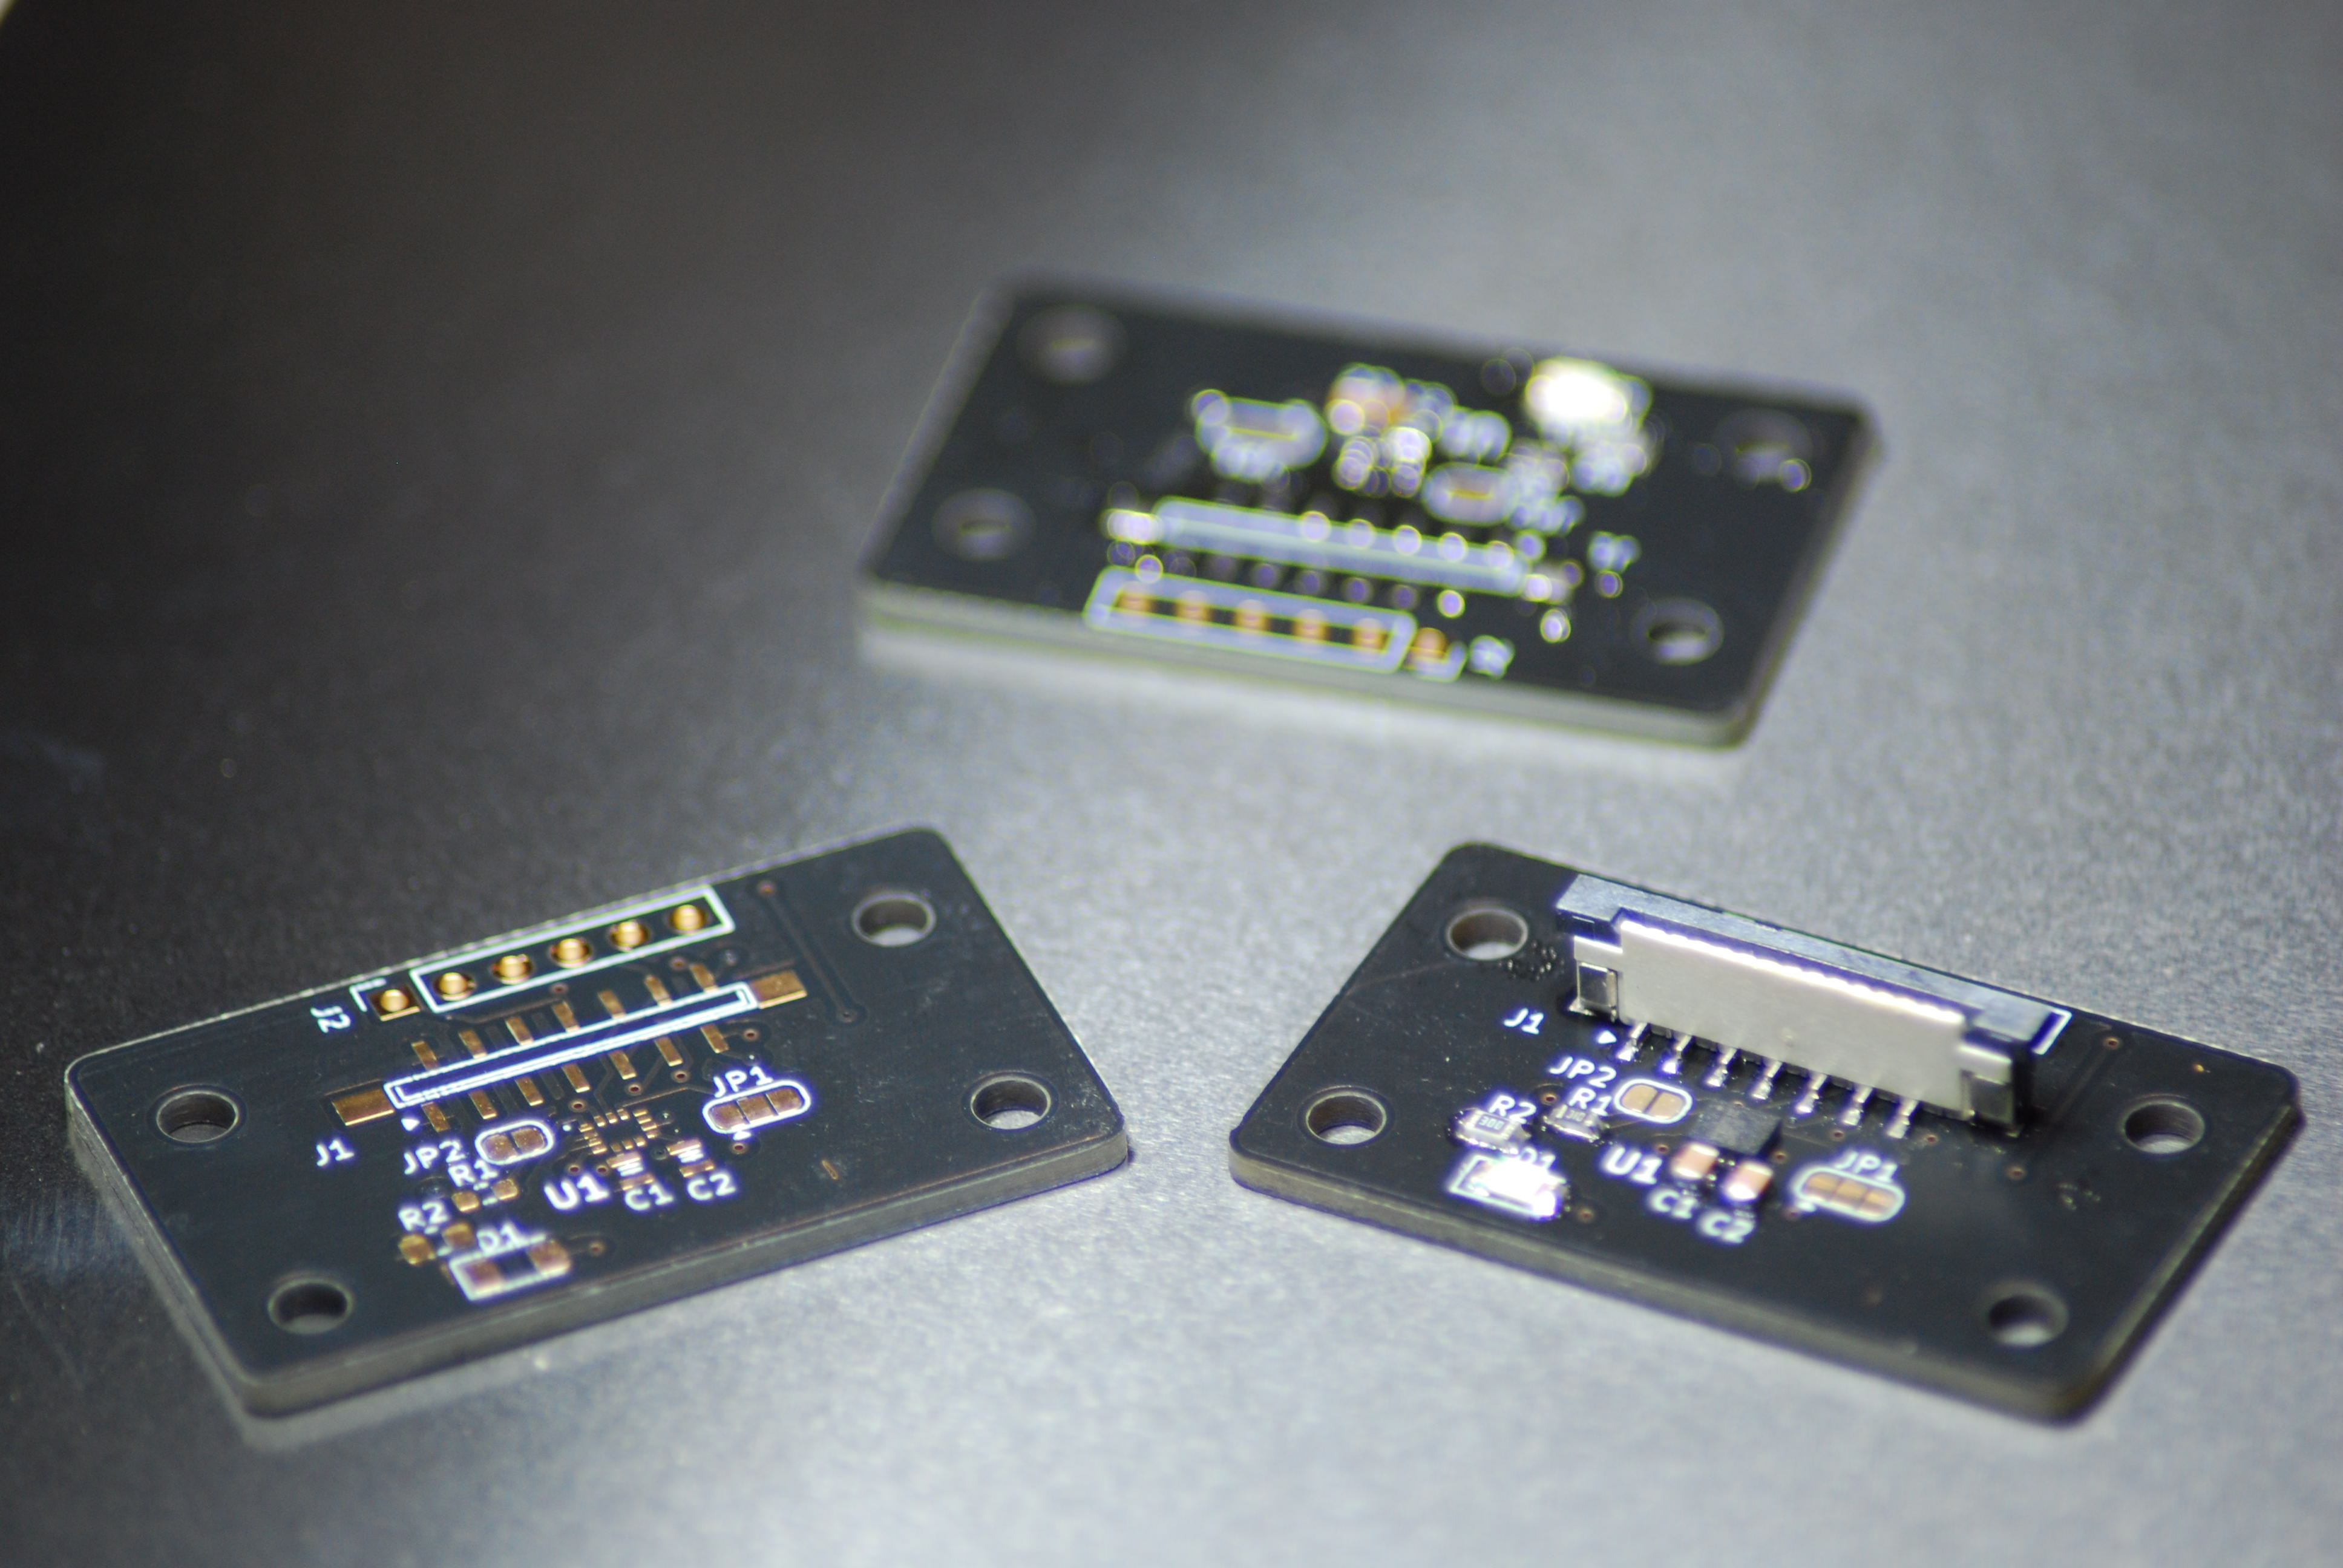
\includegraphics[width=\textwidth]{Image/Accéléromètre haut belle photo.JPG}
					\caption{Accéléromètre du haut}
				\end{figure}
			\end{column}
			\begin{column}{0.35\textwidth}
				\begin{figure}
					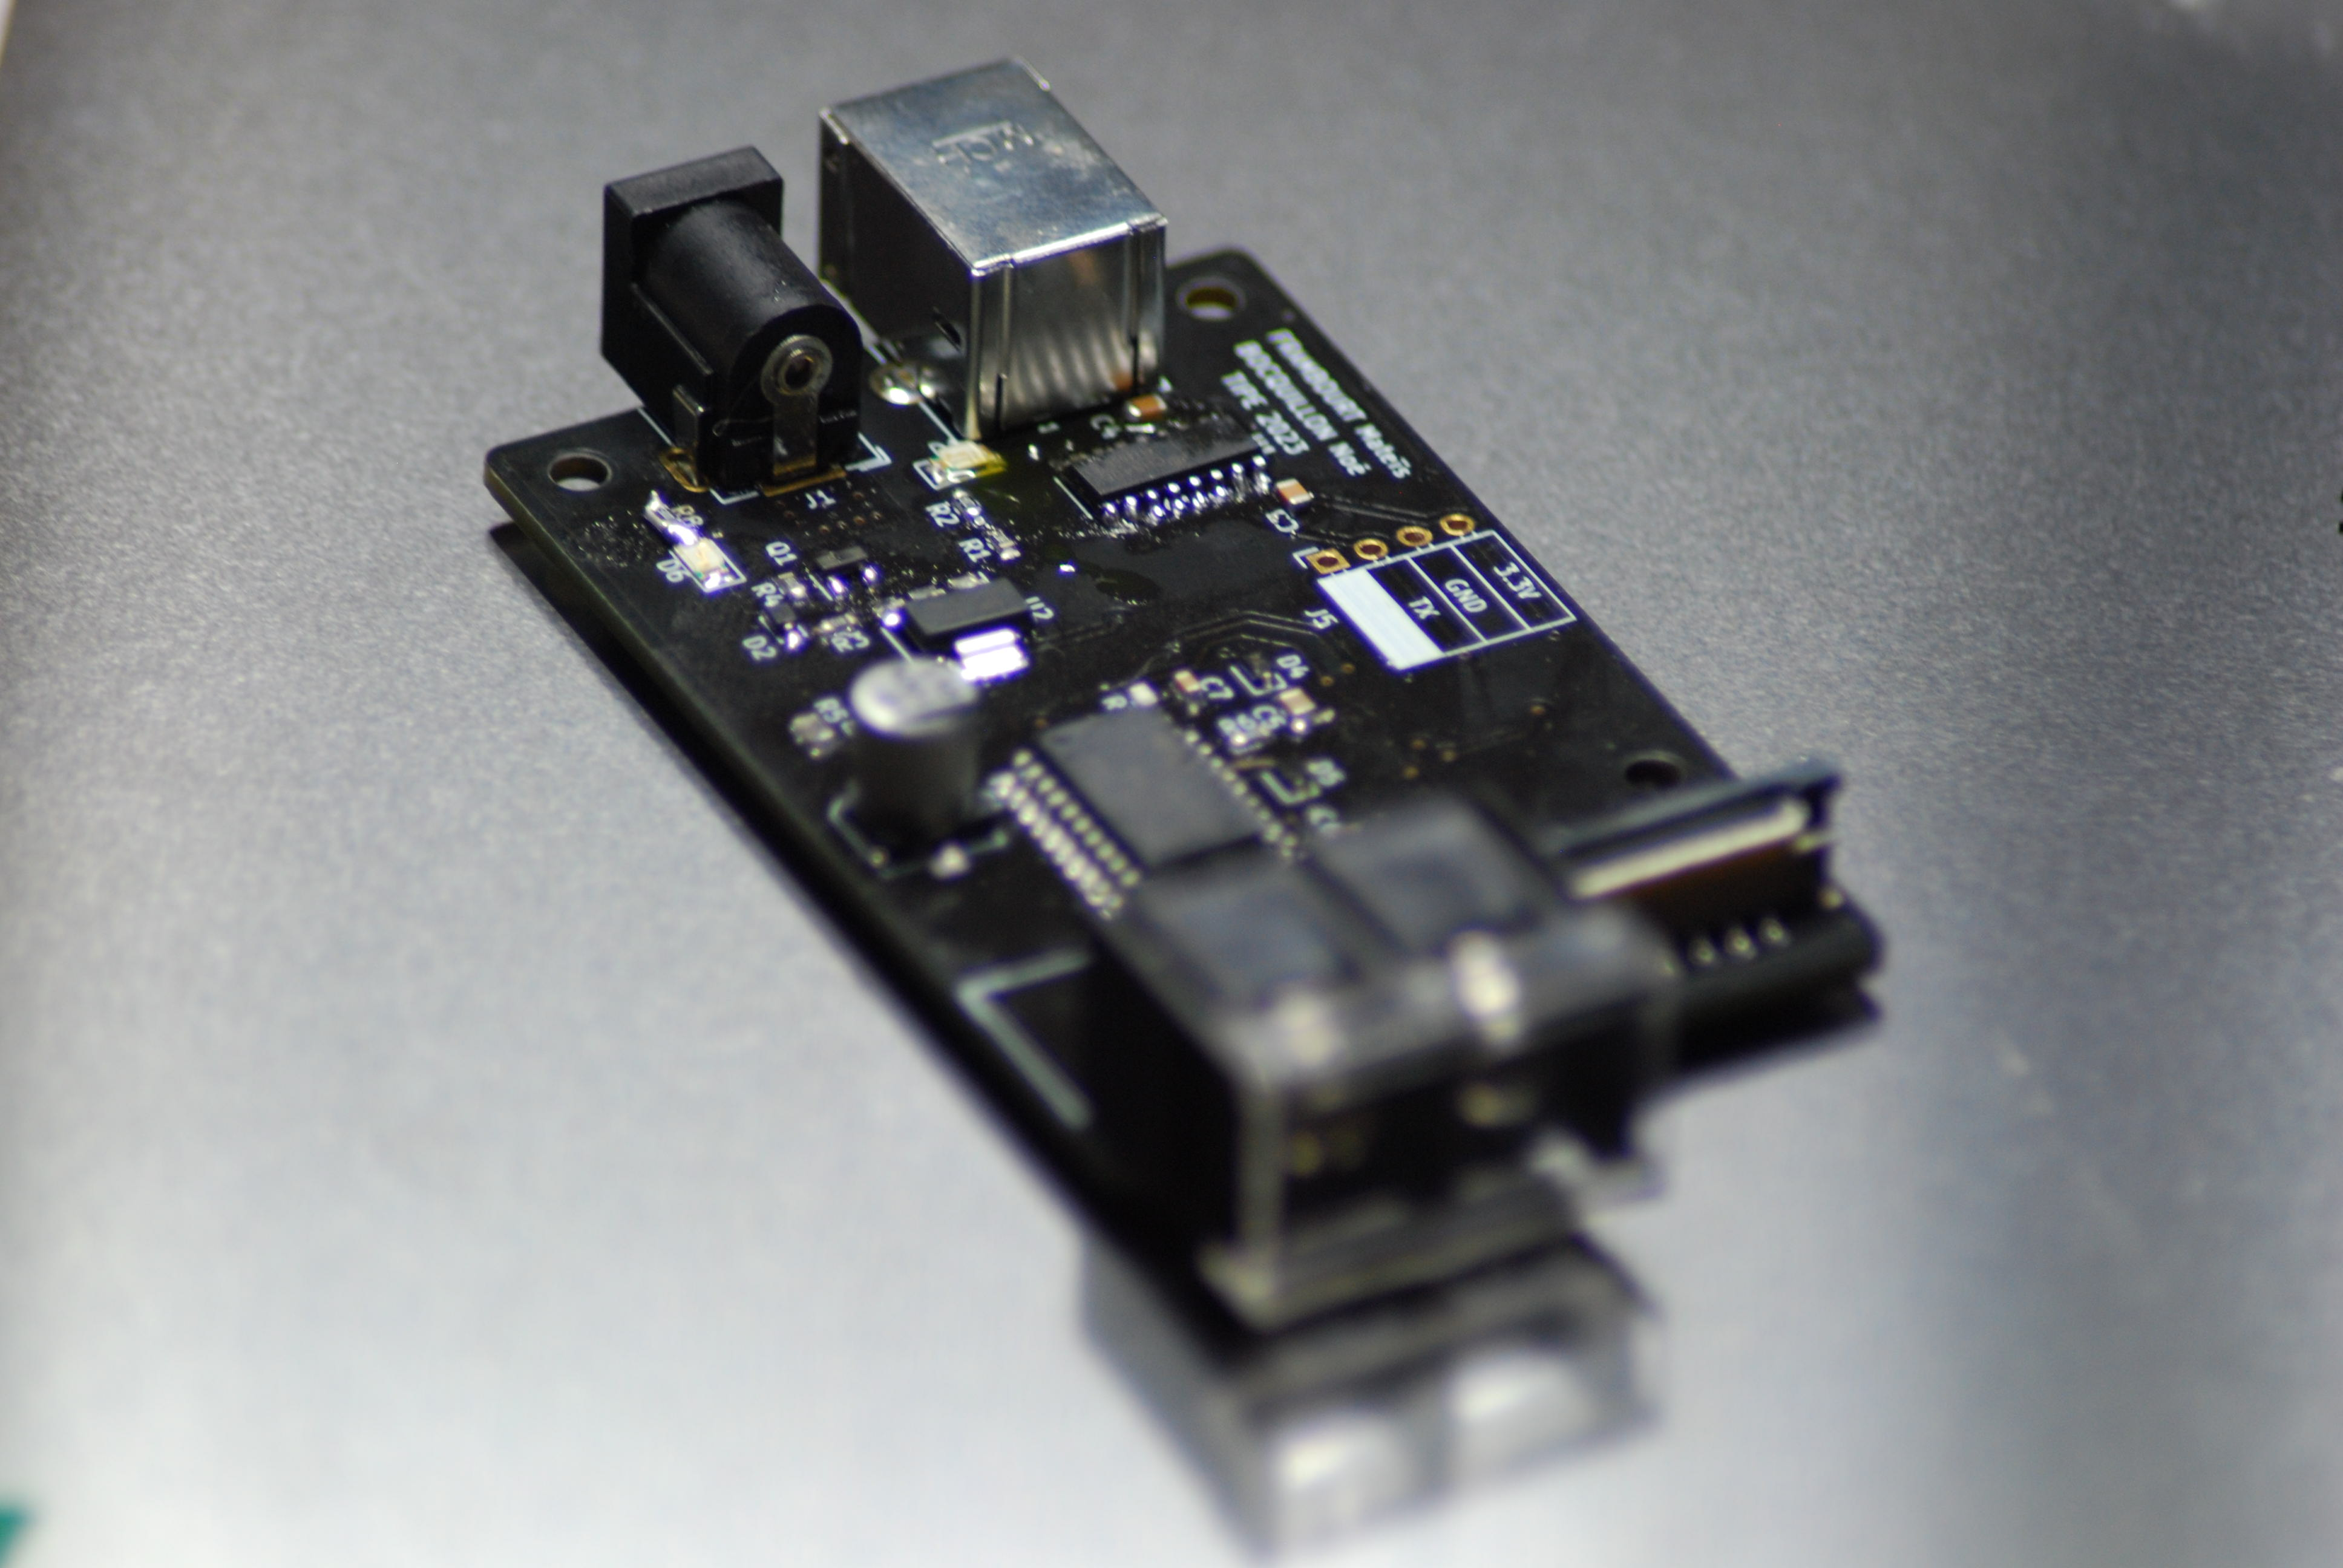
\includegraphics[width=\textwidth]{Image/Carte fixe belle photo.JPG}
					\caption{Carte fixe}
				\end{figure}
			\end{column}
		\end{columns}
	
	\end{frame}
	


	
	\begin{frame}
		Pour les réponses sinusoïdales : 
		\begin{itemize}
			\item Amplitude minimale
			\item Fréquence entre [0.5;5Hz]
			\item Mesure en régime établit 
		\end{itemize}
	\end{frame}
	
	\begin{frame}{Mise en vibration de la maquette}
		\frametitle{Première expérience:Réponse à une excitation sinusoïdale}
		\centering
		\begin{figure}
			
		
		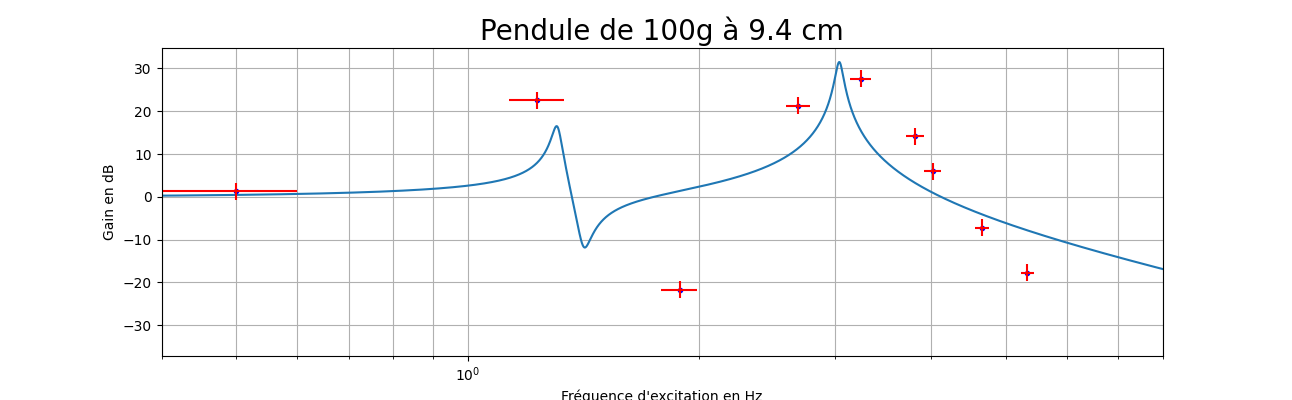
\includegraphics[width=0.8\textwidth]{Image Noé/Données pi avec comparaison (Noé)/Pendule 100g à 9,4 cm.png}
	\caption{Réponse du système à une excitation sinusoïdale pour une masse de 100g à 9.4 cm }
	\end{figure}
\end{frame}
	\begin{frame}
		
		Observations:
		\begin{itemize}
			\item Réduction de l'amplitude des oscillations
			\item Influence du centre de gravité du pendule
			\item Décalage de la fréquence de résonance  
		\end{itemize}
		
	\end{frame}
	
	\begin{frame}{}
		\begin{figure}
			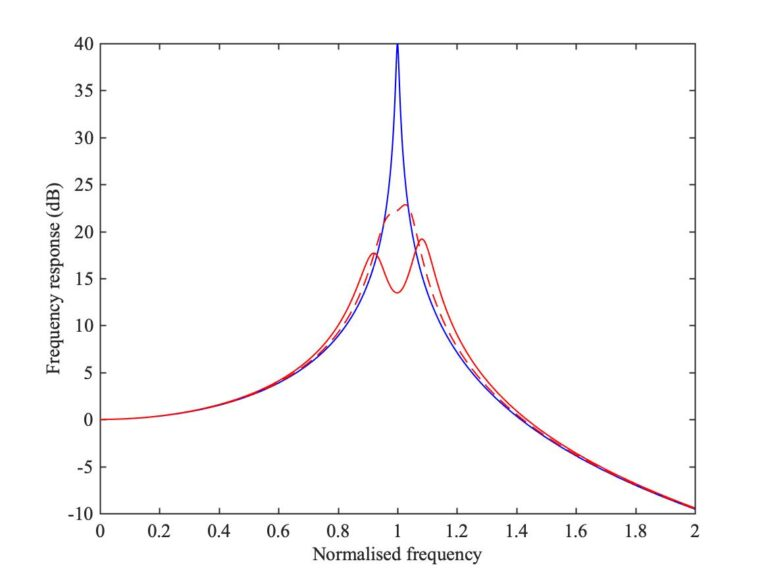
\includegraphics[width=0.8\textwidth]{Image/Objectif en courbe.jpg}
		\end{figure}
	\end{frame}	

	
	\begin{frame}{Mise en vibration de la maquette}
		\frametitle{Première expérience:Réponse à une excitation sinusoïdale}	
		\centering
		\begin{figure}
			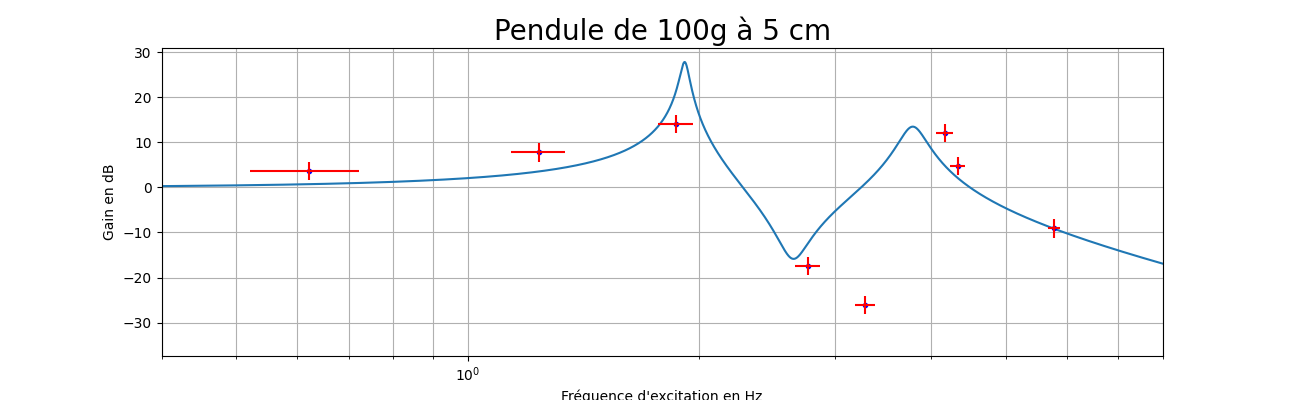
\includegraphics[width=0.7\textwidth]{Image Noé/Données pi avec comparaison (Noé)/Pendule 100g à 5 cm.png}
			\caption{Même réponse en montant la masse à 5cm}
		\end{figure}
			
		\centering
		\begin{figure}
			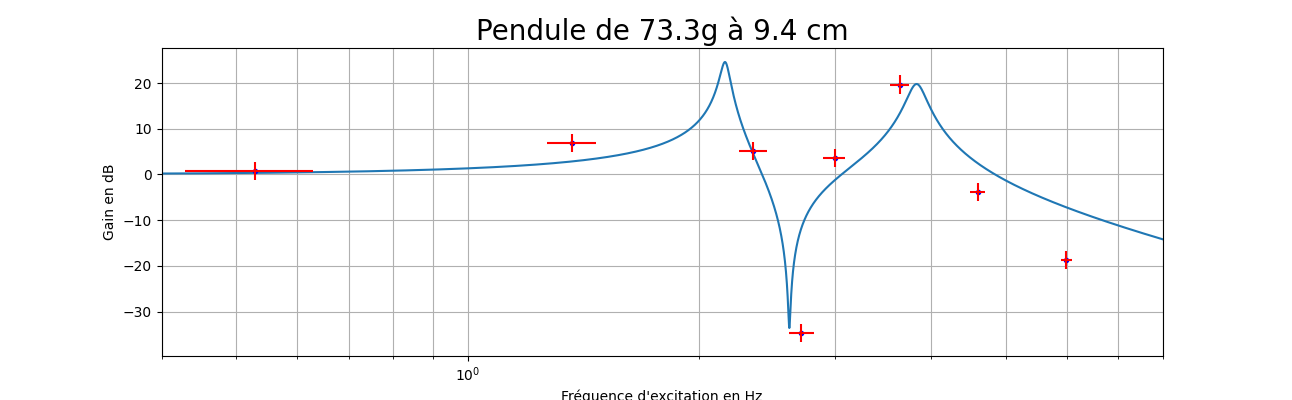
\includegraphics[width=0.7\textwidth]{Image Noé/Données pi avec comparaison (Noé)/Pendule 73.3g à 9,4 cm.png}
			\caption{cette fois çi en prennant 73.3g à 9.4cm}
		\end{figure}
		
		
		
	\end{frame}
	
	
	
	
	\begin{frame}{Mise en vibration de la maquette}
		\frametitle{Deuxième expérience:Dirac}
		\subtitle{bjr}
		\begin{columns}
			\begin{column}{0.5\textwidth}
				\alert{Simulation d'une rafale de vent}
				\begin{figure}
					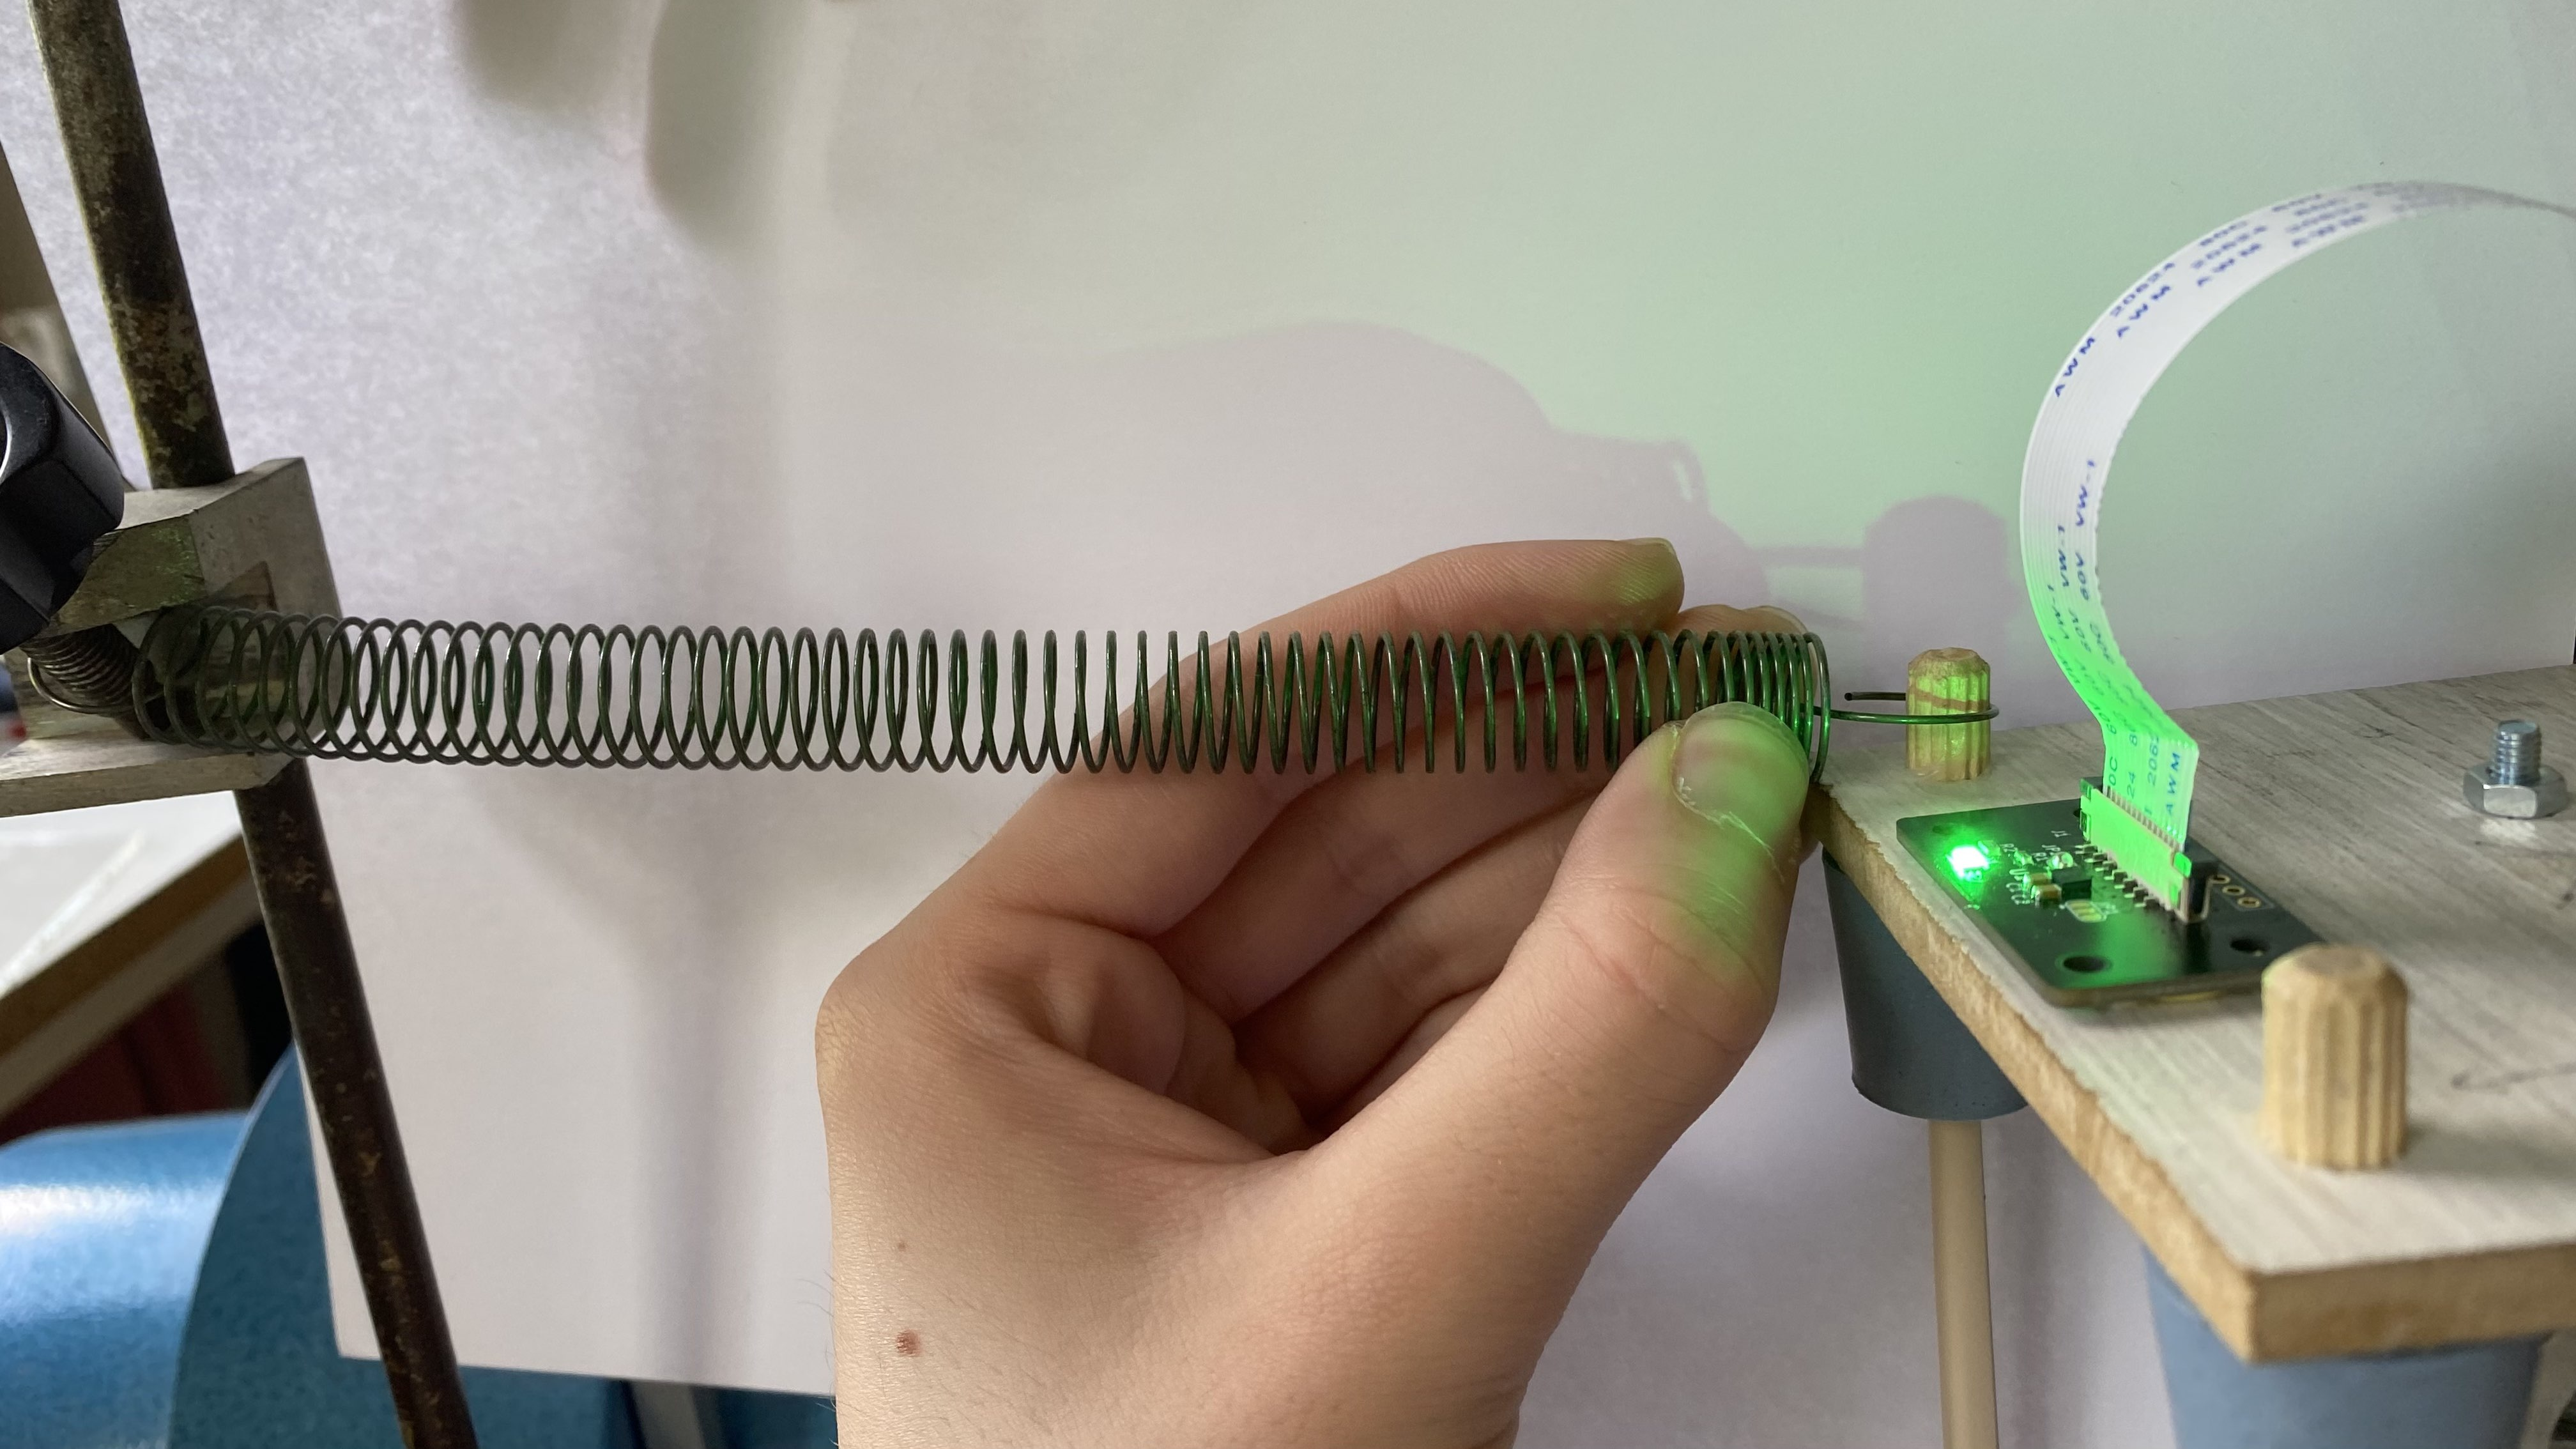
\includegraphics[width=\textwidth]{Image/Montage dirac.jpg}
					\caption{Excitation brève}
				\end{figure}
			\end{column}
			\begin{column}{0.5\textwidth}
				Conditions de l'expérience :
				\begin{itemize}
					\item Dirac avec un ressort 
					\item Oscillations dans un seul plan
				\end{itemize}	
			\end{column}
		\end{columns}
	\end{frame}
	
	
	
	
	\begin{frame}{Mise en vibration de la maquette}
		\frametitle{Deuxième expérience:Réponse à une excitation brève}
		\centering Résultats
		\vspace{12pt}
		\begin{columns}[onlytextwidth]
			\begin{column}{1\textwidth}
				\centering
				\begin{figure}
					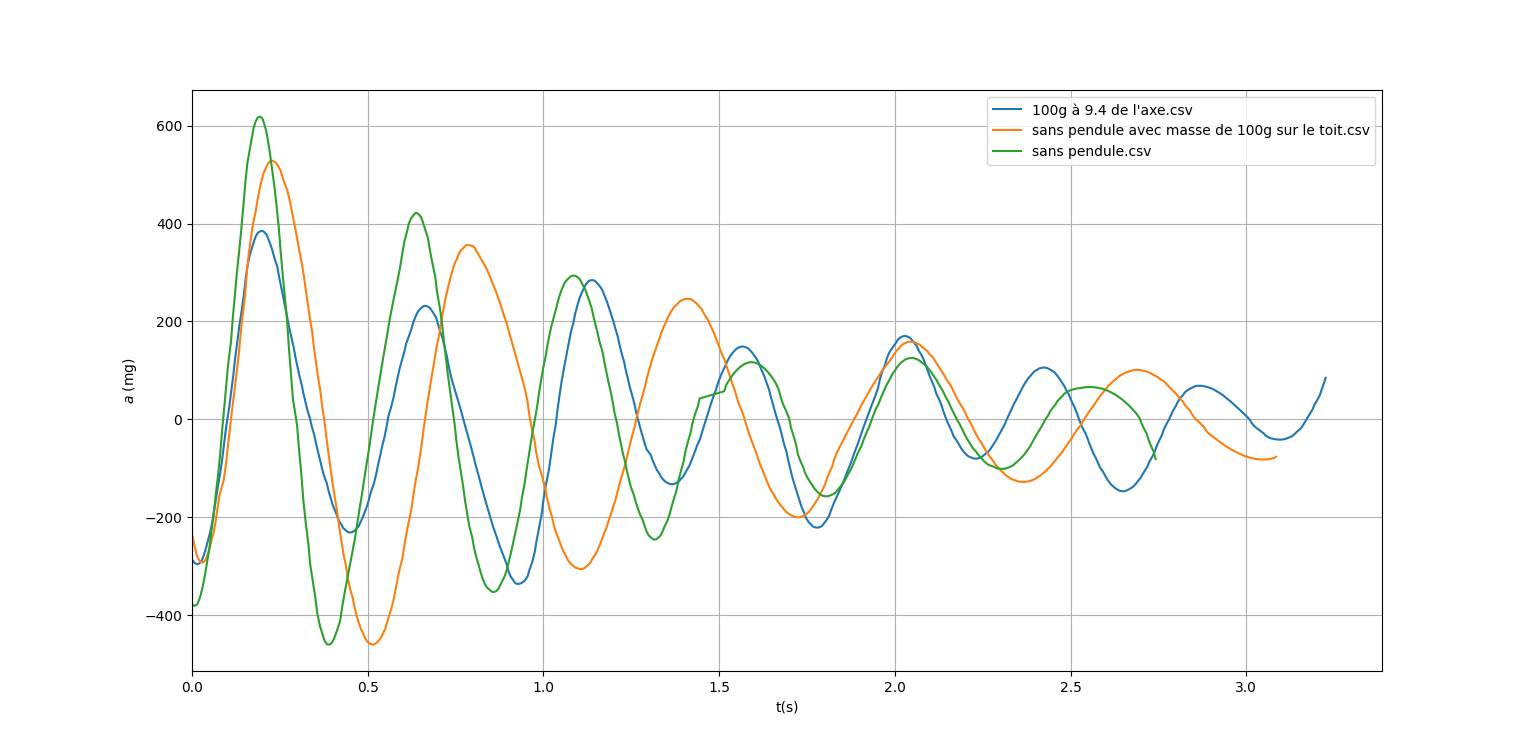
\includegraphics[width=1\textwidth]{Image/Dirac.png}
					\caption{Réponse temporelle à un Dirac}
				\end{figure}
				
			\end{column}
		\end{columns}
		\footnote{A modifier}
	\end{frame}
	
	
	
	
	

	
%	\begin{frame}
	%	contenu...
	
%	$	Mesure de T et de C_{1} expérimentalement :\\ Obtention de la valeur de K$
%	\end{frame}
			
	
	\section{Conclusion}
	
	\begin{frame}{Limites du modèle}
		\begin{itemize}
			\item Dimensions peu assimilables au réel
			\item Élasticité trop importante 
			\item Cependant Résultats comparable au réel.
		\end{itemize}	
		\vspace{12pt}
		
	\end{frame}
	
	%\begin{frame}{explications}
	%dissipation d'énergie dans le pendule , opposition de phases , rapport des pulsations naturelles
	%\end{frame}
	
	%\begin{frame}{limites}
	%	dimension peu adaptées (rapport de la taille et de la masse du pendule par rapport à la structure\\structure trop élastique qui entraine parfois des non linéarité à la fréquence de résonance )
	%\end{frame}
	
	%\begin{frame}{ce qu'on aurait aimé faire}
	%comparaison avec un modèle informatique\\
	%	plus de variations de paramètres\\
	%	mettre le pendule dans un fluide pour plus de viscosité
	%\end{frame}
	
	
	
	
	
	
	%\begin{frame}
	%	\frametitle{Annexe}
	%	Graphique et explication des mesures des coefficients de raideur
	%\end{frame}

	\appendix
	\section*{Annexe}
	\begin{frame}{Caractéristique des TMD en introduction}
		\begin{columns}
			
		
		\begin{column}{0.5\textwidth}
			
		
		\begin{figure}
			\includegraphics[scale=0.4]{Image/Taipeï.jpg}
			\caption{\copyright supertalls.fr} 
		\end{figure}
	\end{column}
	\begin{column}{0.5\textwidth}
		\begin{itemize}
			\item Masse: 660 Tonnes
			\item diamètre: 5,5m
			\item amplitude maximale : 1,5m 
			\item amortissement: jusqu'à 40\% maximum
			\item prix : 4 millions de dollars
		\end{itemize}
	\end{column}

\end{columns}
	\end{frame}

	\begin{frame}{Caractéristique des TMD en introduction}
		\begin{columns}
			\begin{column}{0.5\textwidth}
				\begin{figure}
					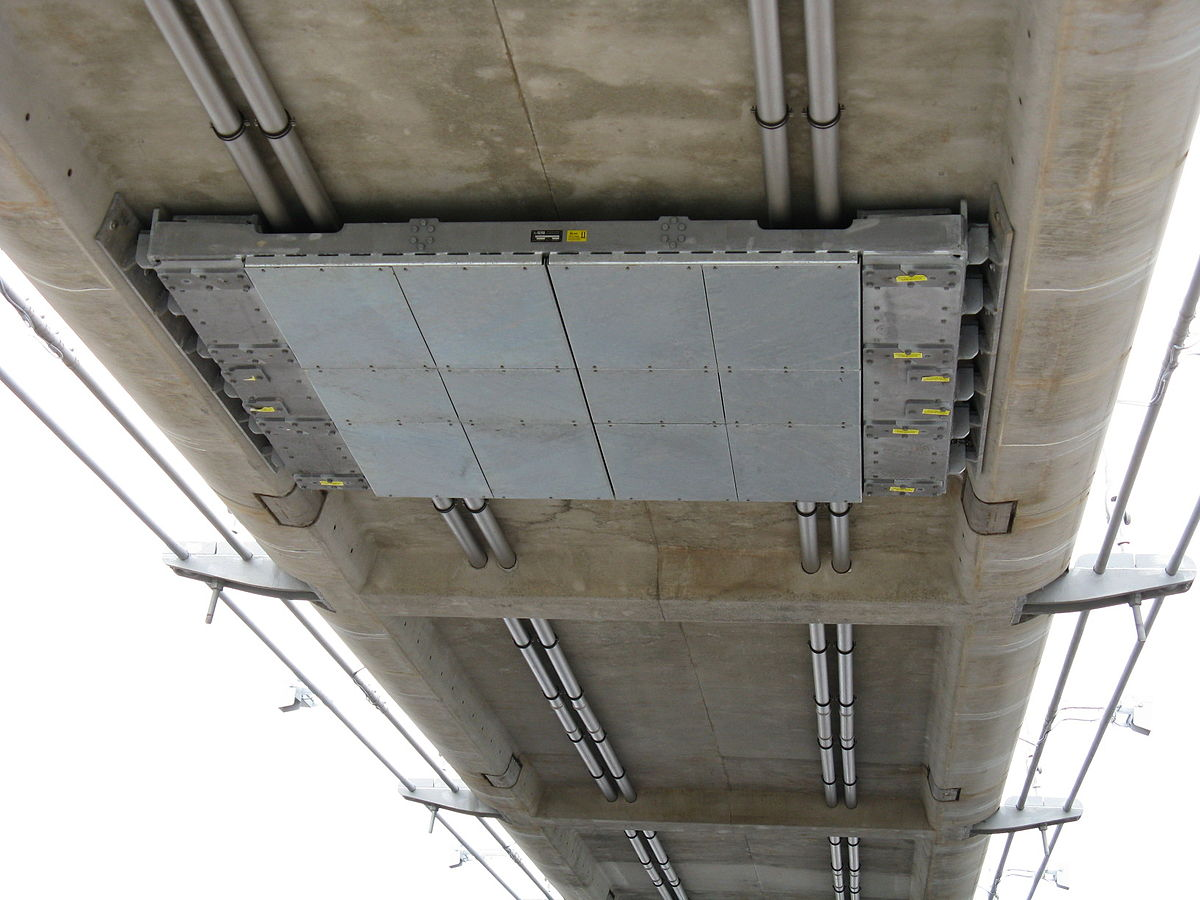
\includegraphics[width=\textwidth]{Image/TMD pont.jpg}
					\caption{\copyright JohnYeadon}
				\end{figure}
			\end{column}
			\begin{column}{0.5\textwidth}
				\begin{itemize}
					\item Localisation : Stockton-on-Tees
					\item Masse : 700 Kg
					\item Nombre : 7 sur l'entiereté du pont
				\end{itemize}
			\end{column}
			
		\end{columns}
	\end{frame}
	\begin{frame}{Accéléromètre utilisé}
		\begin{columns}
			\begin{column}{0.5\textwidth}
				\begin{figure}
					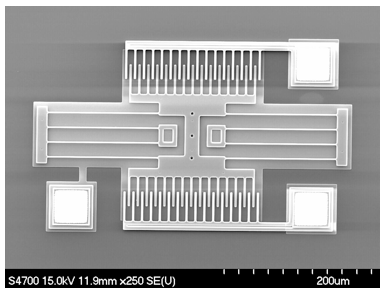
\includegraphics[width=\textwidth]{Image/microsensor_microactuator.png}
					\caption{\copyright www.mems-exchange.org}
				\end{figure}
			\end{column}
			\begin{column}{0.5\textwidth}
				\begin{itemize}
					\item LSM6DS3
					\item 6 degré de liberté 
					\item $\pm 2$/$\pm 16$ g
					\item $U(a)=0.122$ mg 
					\item $N(a) = 90 \frac{\mu g}{\sqrt{Hz}}$ 
				\end{itemize}
			\end{column}
			
		\end{columns}
	\end{frame}
	\begin{frame}{Caractéristique du raspberry pi pico W} 
		\begin{columns}
			\begin{column}{0.5\textwidth}
				\begin{figure}
					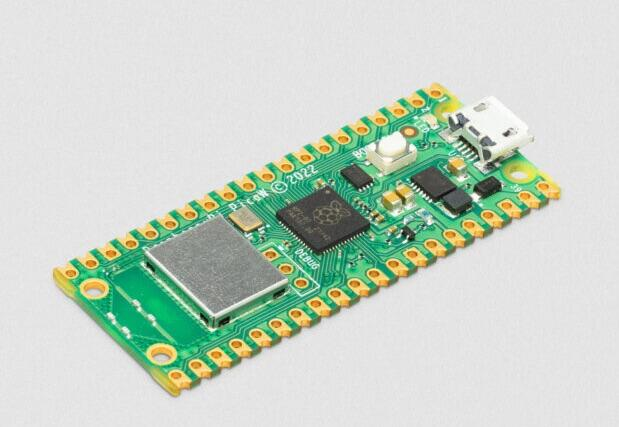
\includegraphics[width=\textwidth]{Image/pico w.jpg}
					\caption{Pico W}
				\end{figure}
			\end{column}
			\begin{column}{0.5\textwidth}
				\begin{itemize}
					\item Programmable en C++/Python 
					\item 15€ 
					\item 2 Coeurs M0+ 133 MHz 
					\item FPU integré
					\item Wifi 2.4 GHz
				\end{itemize}
			\end{column}
		\end{columns}
		
	\end{frame}
	\begin{frame}{Circuit imprimé fixe}
		\begin{columns}
			\begin{column}{0.5\textwidth}
				\begin{figure}
					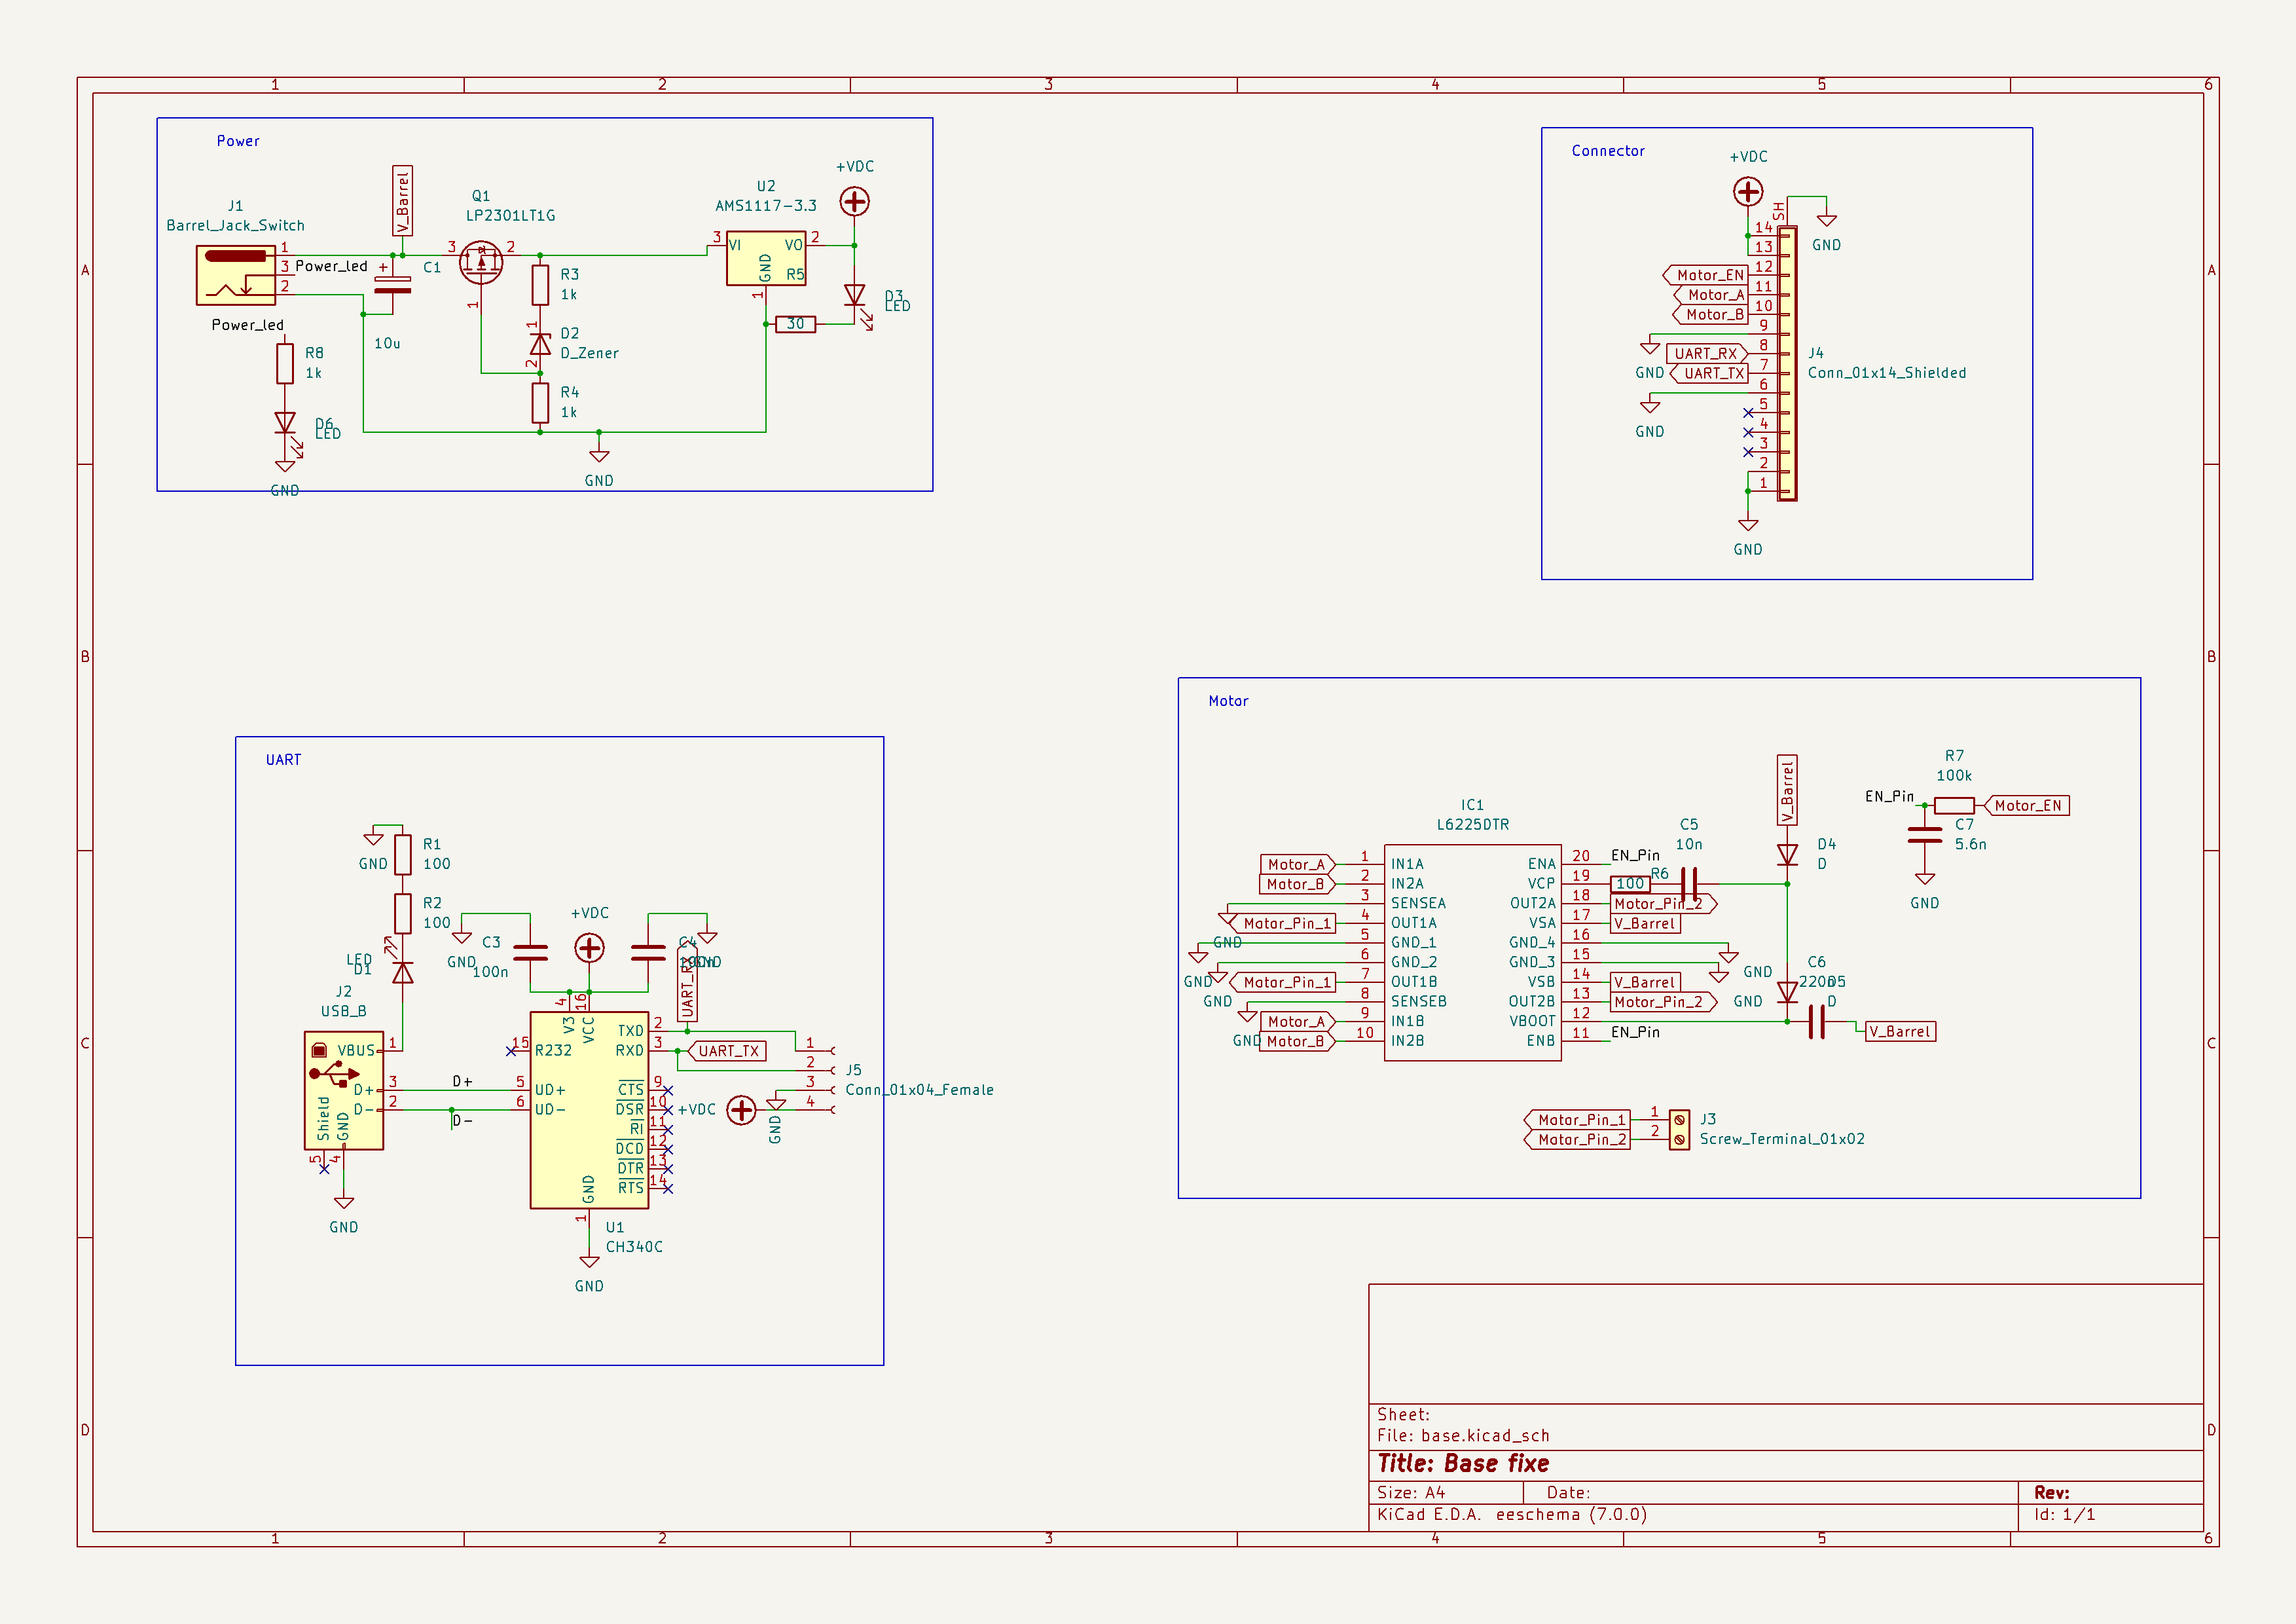
\includegraphics[width=\textwidth]{Image/base fixe.png}
					\caption{branchement base fixe}
				\end{figure}
			\end{column}
			\begin{column}{0.5\textwidth}
				\begin{figure}
					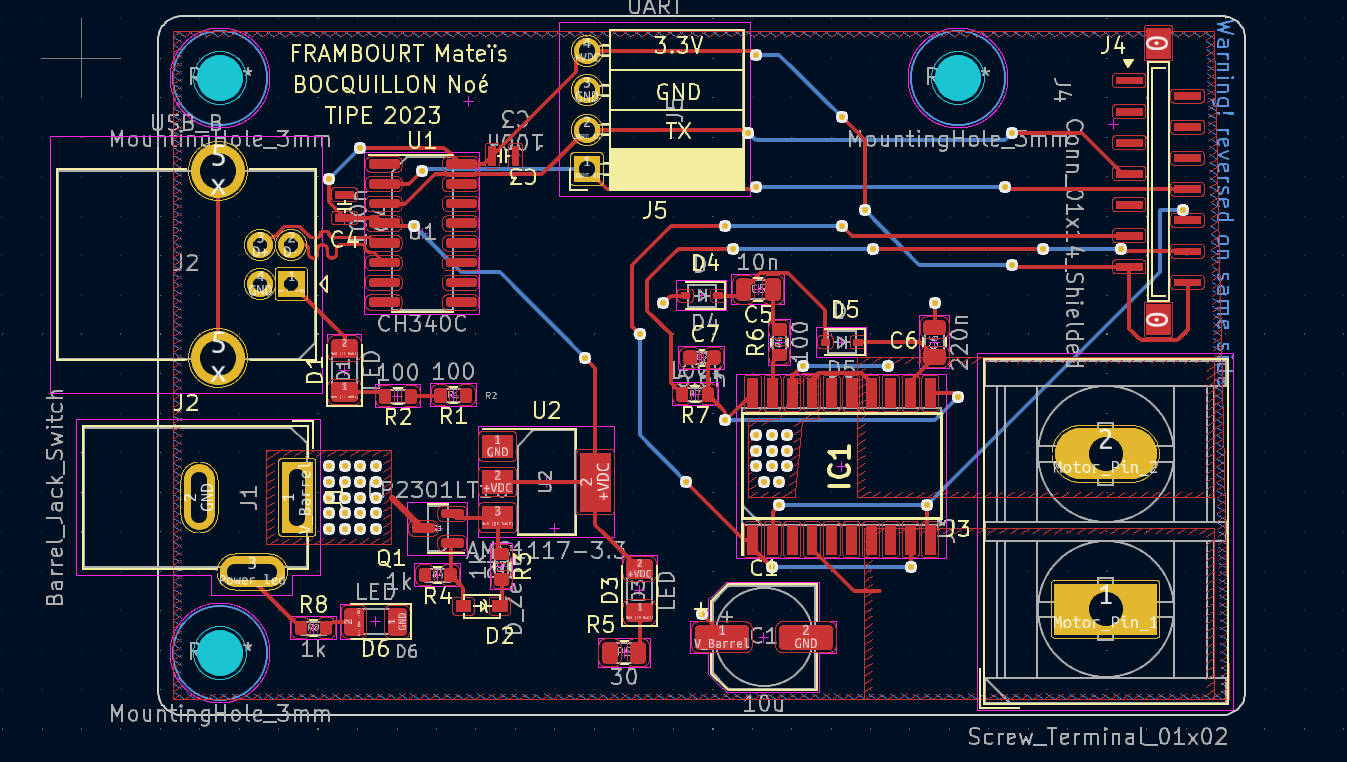
\includegraphics[width=\textwidth]{Image/Base fixe pcb.png}
					\caption{PCB base fixe}
				\end{figure}
			\end{column}
		\end{columns}
	\end{frame}
	\begin{frame}{Circuit imprimé principal}
		\begin{columns}
			\begin{column}{0.5\textwidth}
				\begin{figure}
					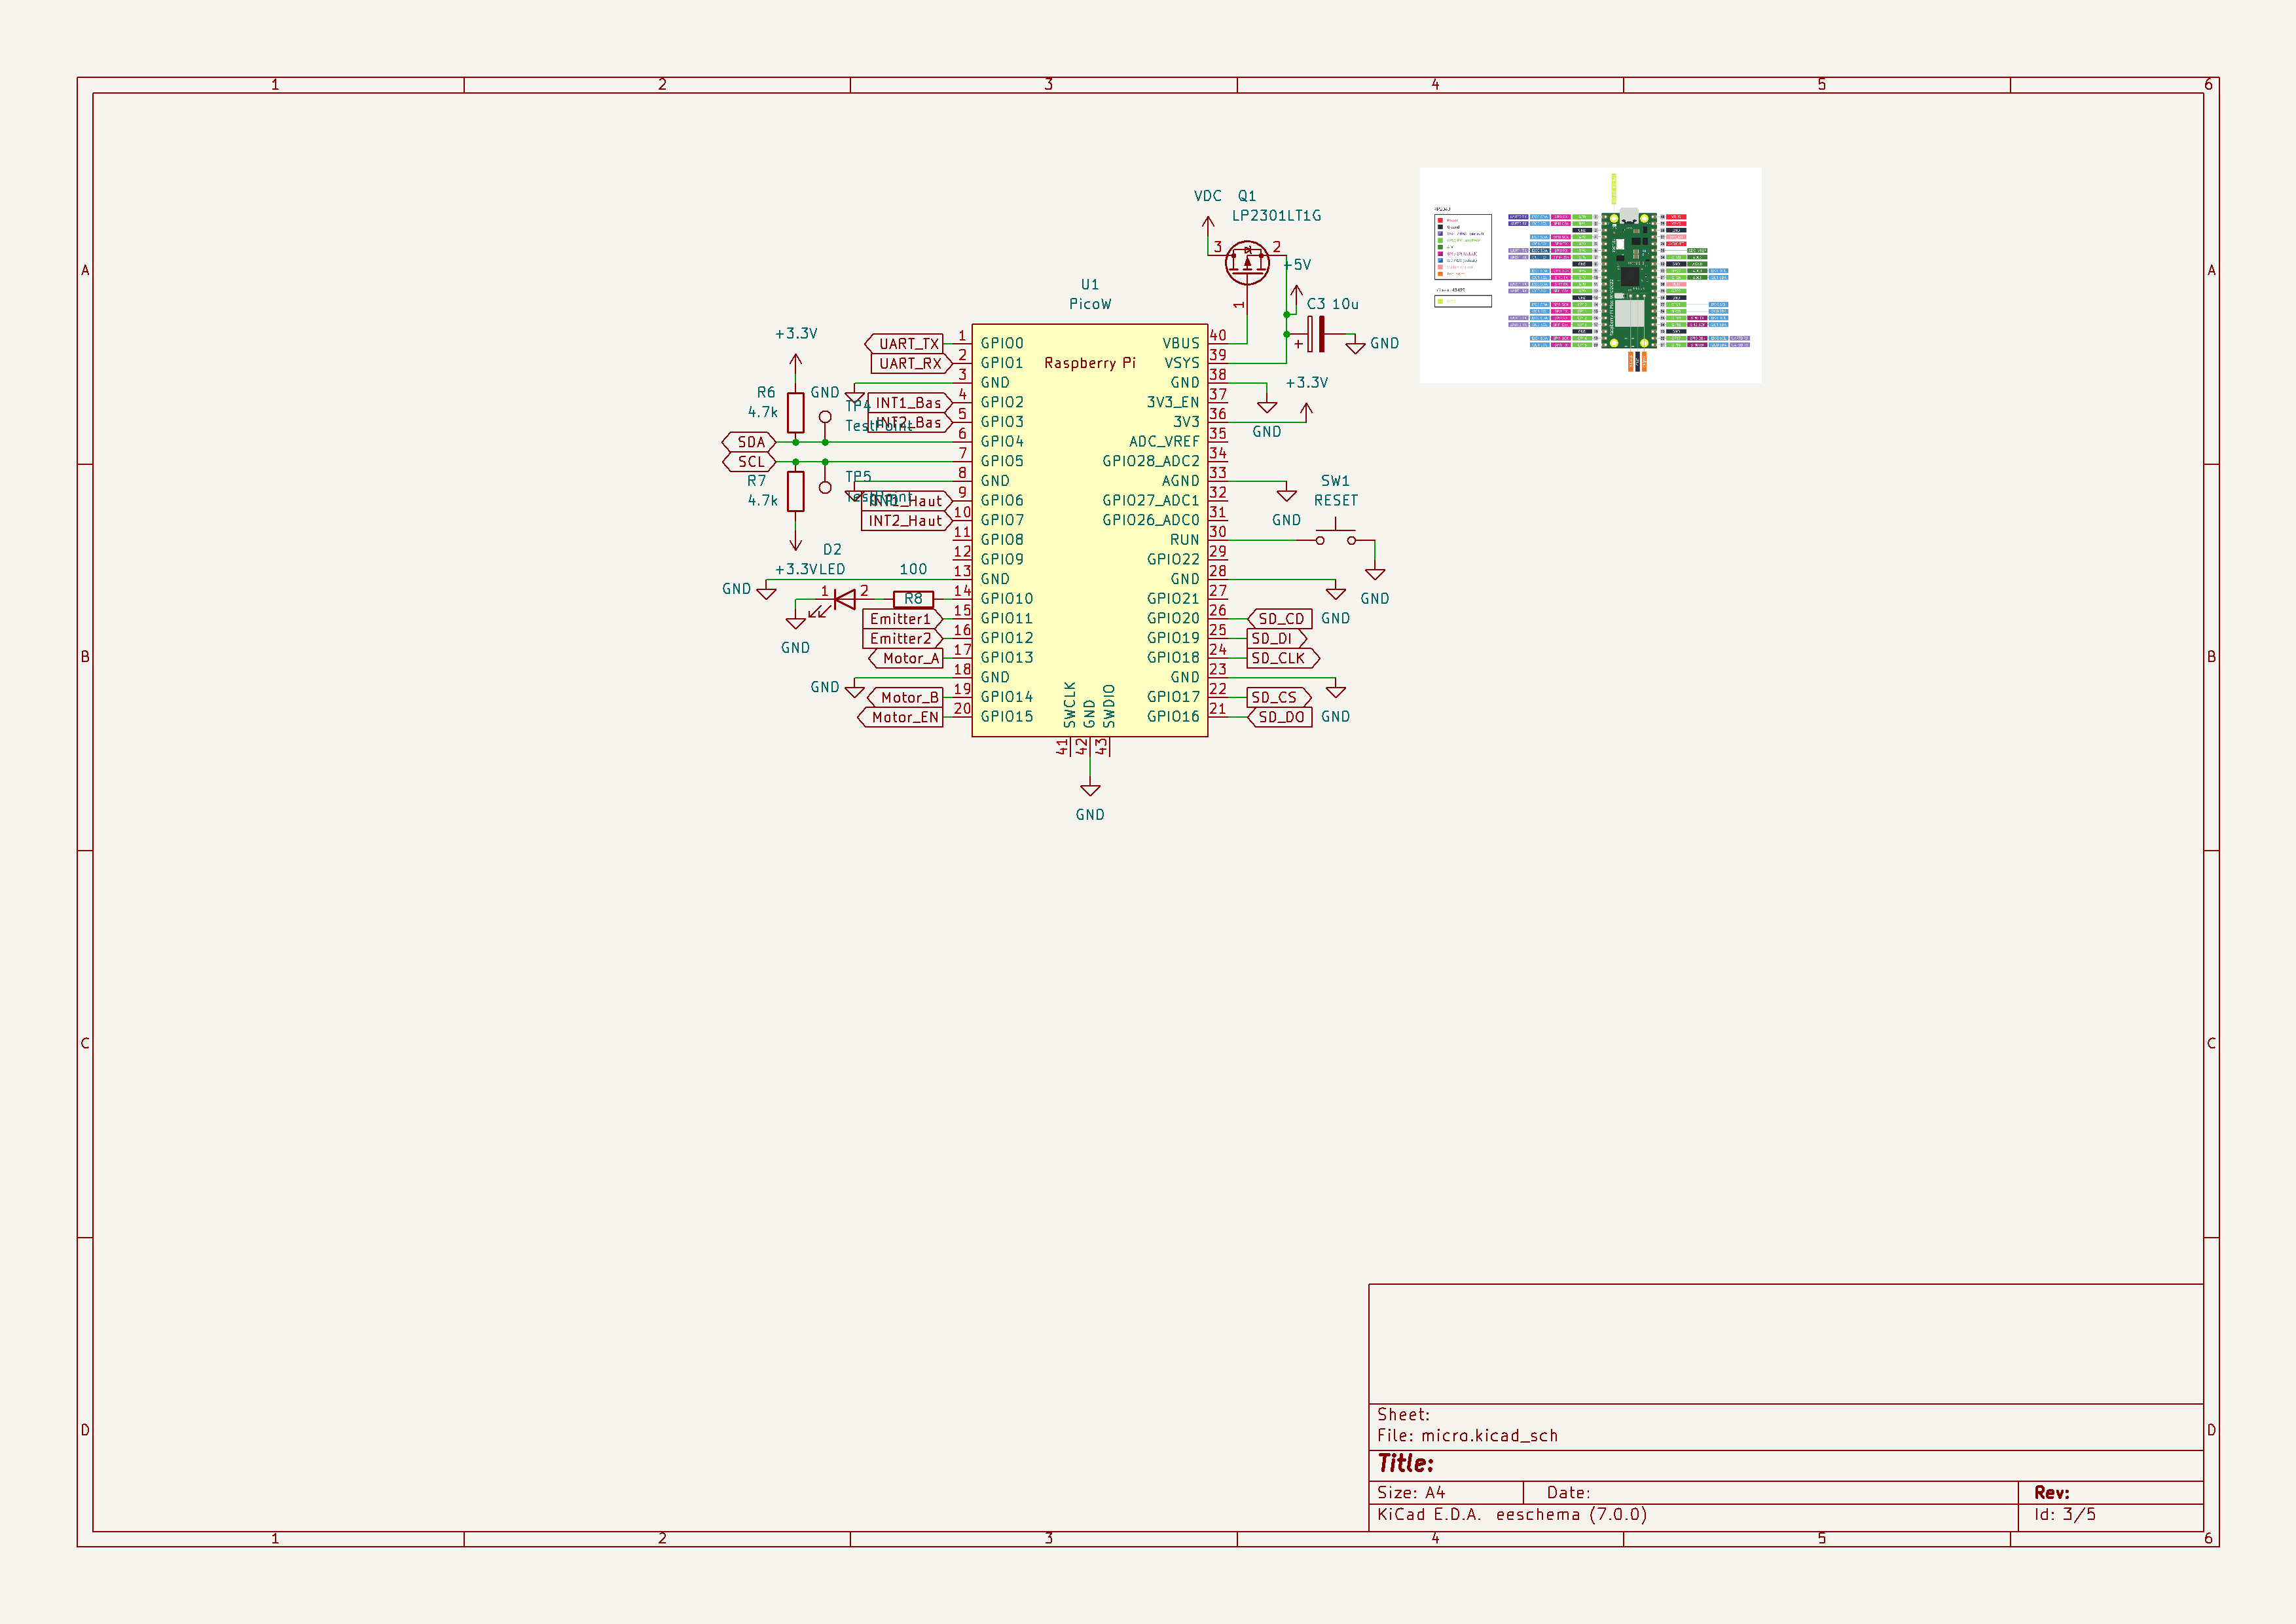
\includegraphics[width=\textwidth]{Image/SCH MAINboard mcu.png}
					\caption{Branchement Carte mère }
				\end{figure}
			\end{column}
			\begin{column}{0.5\textwidth}
				\begin{figure}
					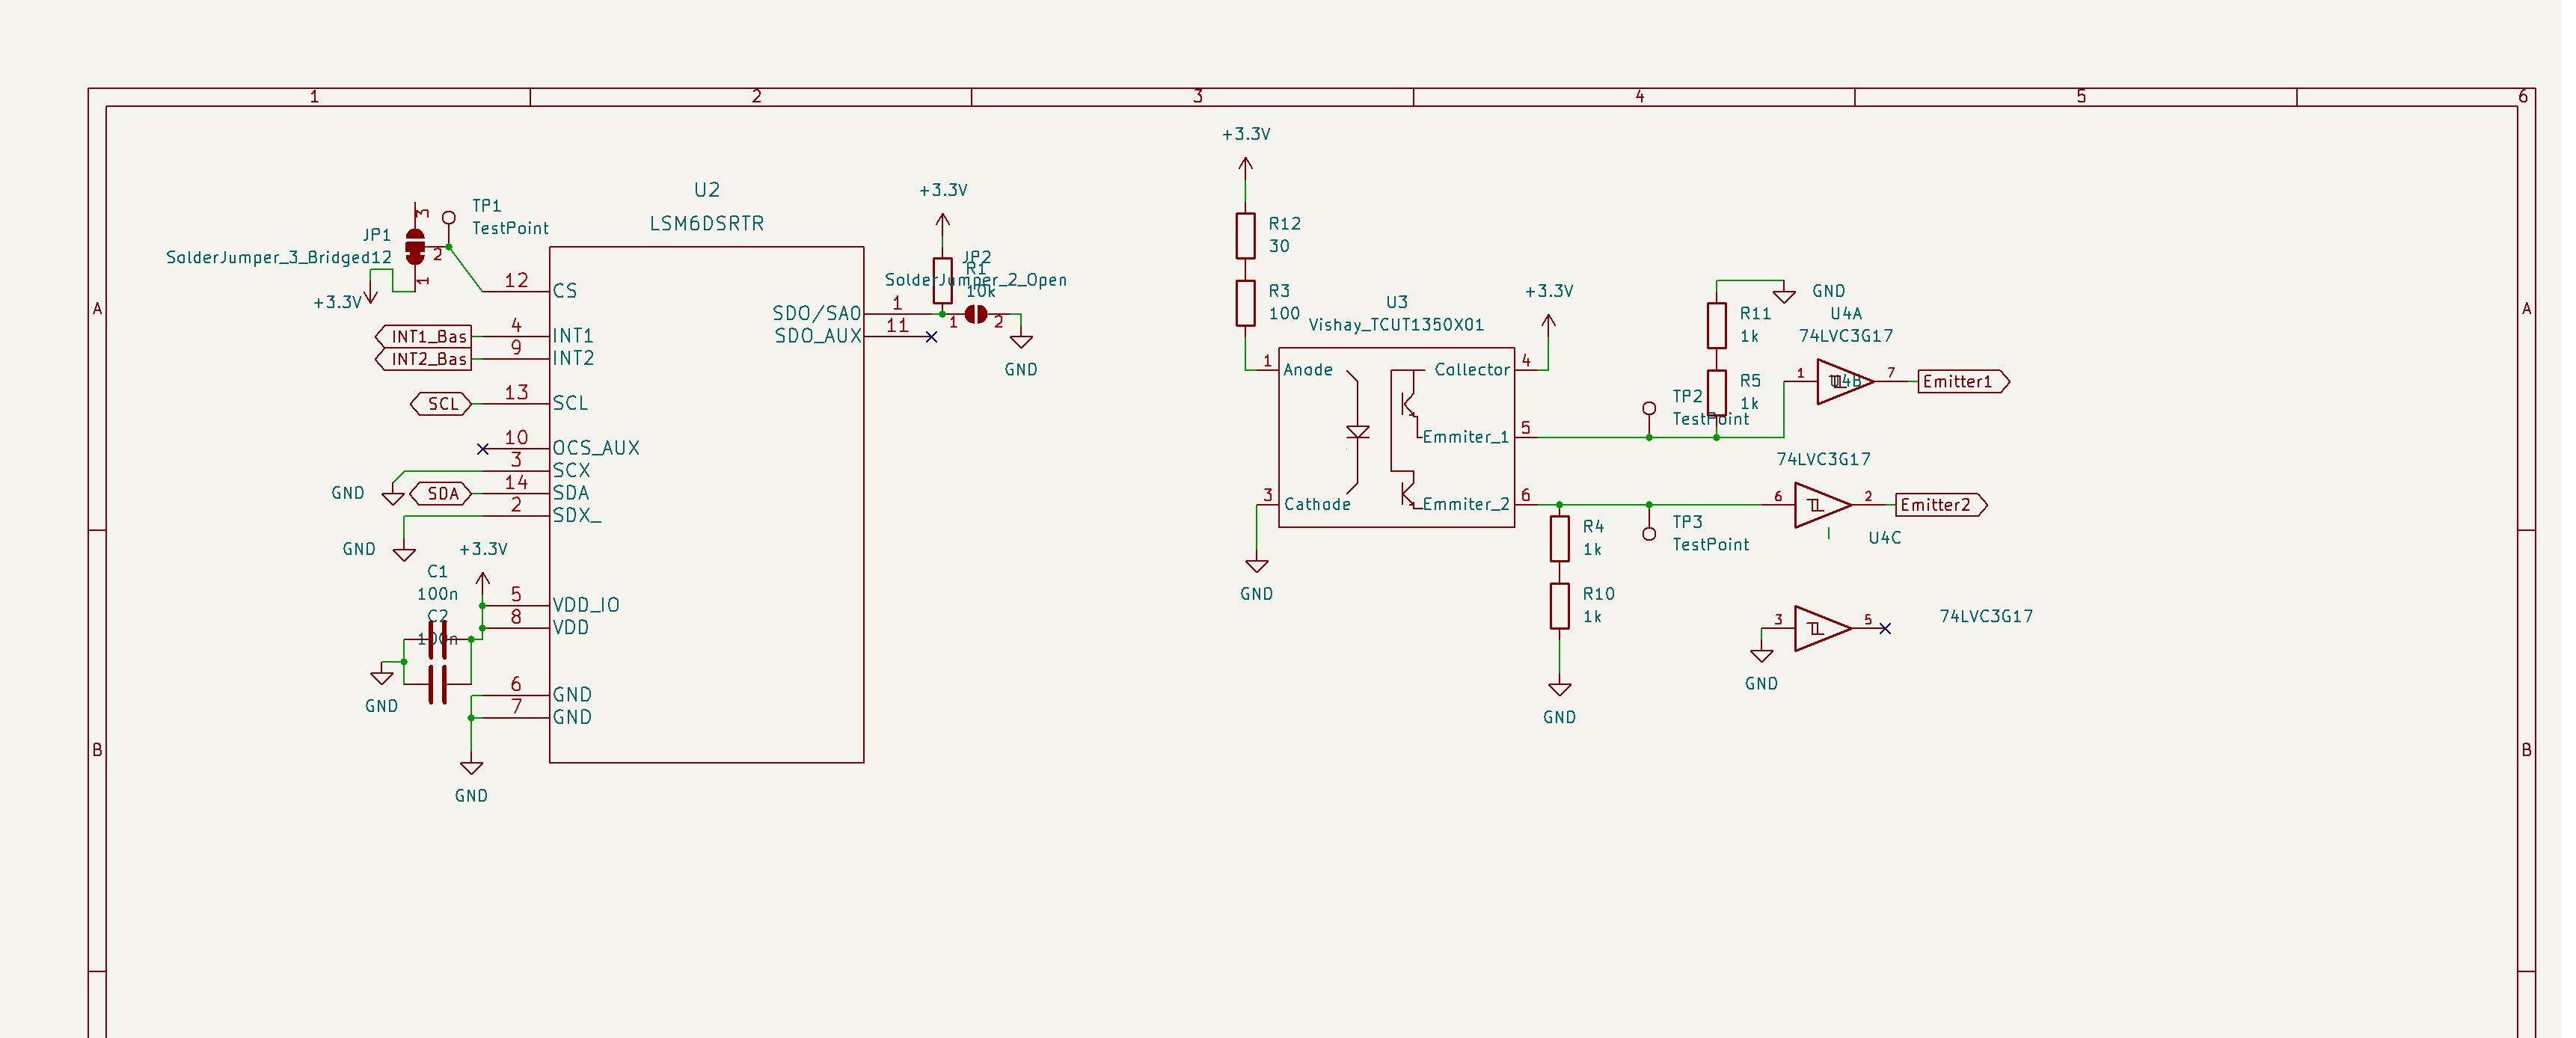
\includegraphics[width=\textwidth]{Image/Sch mainboard sensor.png}
					\caption{Capteur de la carte mère}
				\end{figure}
			\end{column}
		\end{columns}
	\end{frame}
	\begin{frame}{Schéma PCB}
		\begin{figure}
			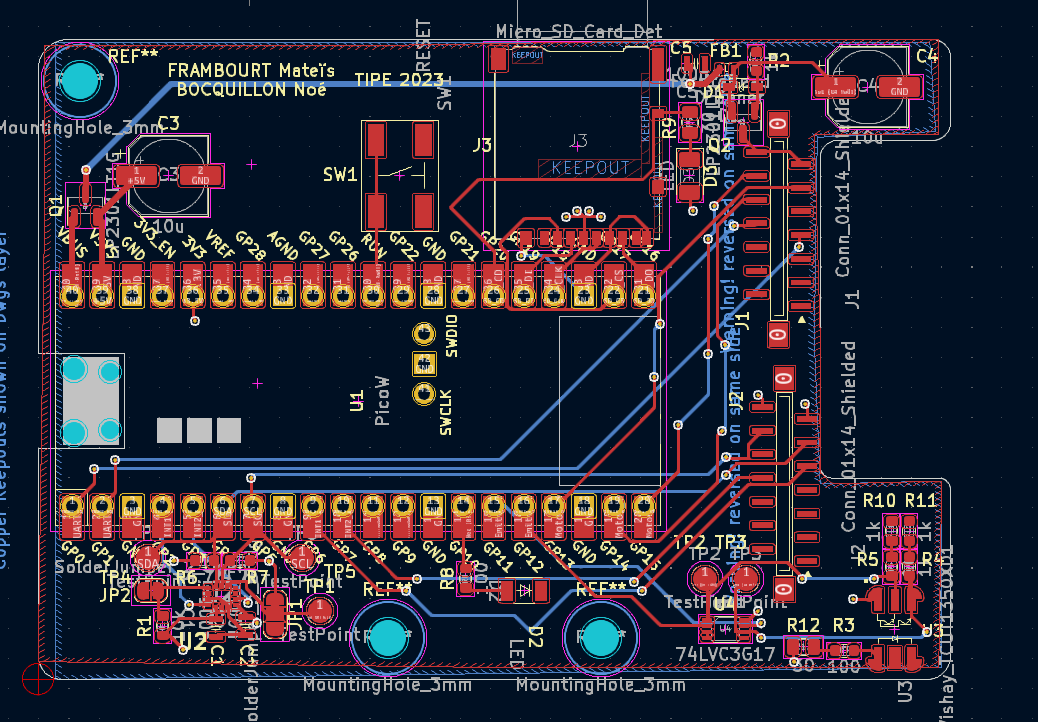
\includegraphics[width=0.8\textwidth]{Image/mb pcb.png}
			\caption{PCB carte mère}
		\end{figure}
	\end{frame}
\end{document} 